\documentclass[twoside]{book}

% Packages required by doxygen
\usepackage{fixltx2e}
\usepackage{calc}
\usepackage{doxygen}
\usepackage[export]{adjustbox} % also loads graphicx
\usepackage{graphicx}
\usepackage[utf8]{inputenc}
\usepackage{makeidx}
\usepackage{multicol}
\usepackage{multirow}
\PassOptionsToPackage{warn}{textcomp}
\usepackage{textcomp}
\usepackage[nointegrals]{wasysym}
\usepackage[table]{xcolor}

% Font selection
\usepackage[T1]{fontenc}
\usepackage[scaled=.90]{helvet}
\usepackage{courier}
\usepackage{amssymb}
\usepackage{sectsty}
\renewcommand{\familydefault}{\sfdefault}
\allsectionsfont{%
  \fontseries{bc}\selectfont%
  \color{darkgray}%
}
\renewcommand{\DoxyLabelFont}{%
  \fontseries{bc}\selectfont%
  \color{darkgray}%
}
\newcommand{\+}{\discretionary{\mbox{\scriptsize$\hookleftarrow$}}{}{}}

% Page & text layout
\usepackage{geometry}
\geometry{%
  a4paper,%
  top=2.5cm,%
  bottom=2.5cm,%
  left=2.5cm,%
  right=2.5cm%
}
\tolerance=750
\hfuzz=15pt
\hbadness=750
\setlength{\emergencystretch}{15pt}
\setlength{\parindent}{0cm}
\setlength{\parskip}{3ex plus 2ex minus 2ex}
\makeatletter
\renewcommand{\paragraph}{%
  \@startsection{paragraph}{4}{0ex}{-1.0ex}{1.0ex}{%
    \normalfont\normalsize\bfseries\SS@parafont%
  }%
}
\renewcommand{\subparagraph}{%
  \@startsection{subparagraph}{5}{0ex}{-1.0ex}{1.0ex}{%
    \normalfont\normalsize\bfseries\SS@subparafont%
  }%
}
\makeatother

% Headers & footers
\usepackage{fancyhdr}
\pagestyle{fancyplain}
\fancyhead[LE]{\fancyplain{}{\bfseries\thepage}}
\fancyhead[CE]{\fancyplain{}{}}
\fancyhead[RE]{\fancyplain{}{\bfseries\leftmark}}
\fancyhead[LO]{\fancyplain{}{\bfseries\rightmark}}
\fancyhead[CO]{\fancyplain{}{}}
\fancyhead[RO]{\fancyplain{}{\bfseries\thepage}}
\fancyfoot[LE]{\fancyplain{}{}}
\fancyfoot[CE]{\fancyplain{}{}}
\fancyfoot[RE]{\fancyplain{}{\bfseries\scriptsize Generated by Doxygen }}
\fancyfoot[LO]{\fancyplain{}{\bfseries\scriptsize Generated by Doxygen }}
\fancyfoot[CO]{\fancyplain{}{}}
\fancyfoot[RO]{\fancyplain{}{}}
\renewcommand{\footrulewidth}{0.4pt}
\renewcommand{\chaptermark}[1]{%
  \markboth{#1}{}%
}
\renewcommand{\sectionmark}[1]{%
  \markright{\thesection\ #1}%
}

% Indices & bibliography
\usepackage{natbib}
\usepackage[titles]{tocloft}
\setcounter{tocdepth}{3}
\setcounter{secnumdepth}{5}
\makeindex

% Hyperlinks (required, but should be loaded last)
\usepackage{ifpdf}
\ifpdf
  \usepackage[pdftex,pagebackref=true]{hyperref}
\else
  \usepackage[ps2pdf,pagebackref=true]{hyperref}
\fi
\hypersetup{%
  colorlinks=true,%
  linkcolor=blue,%
  citecolor=blue,%
  unicode%
}

% Custom commands
\newcommand{\clearemptydoublepage}{%
  \newpage{\pagestyle{empty}\cleardoublepage}%
}

\usepackage{caption}
\captionsetup{labelsep=space,justification=centering,font={bf},singlelinecheck=off,skip=4pt,position=top}

%===== C O N T E N T S =====

\begin{document}

% Titlepage & ToC
\hypersetup{pageanchor=false,
             bookmarksnumbered=true,
             pdfencoding=unicode
            }
\pagenumbering{roman}
\begin{titlepage}
\vspace*{7cm}
\begin{center}%
{\Large E\+E445\+M/\+E\+E380L Lab 2 Documentation }\\
\vspace*{1cm}
{\large Generated by Doxygen 1.8.11}\\
\end{center}
\end{titlepage}
\clearemptydoublepage
\tableofcontents
\clearemptydoublepage
\pagenumbering{arabic}
\hypersetup{pageanchor=true}

%--- Begin generated contents ---
\chapter{Data Structure Index}
\section{Data Structures}
Here are the data structures with brief descriptions\+:\begin{DoxyCompactList}
\item\contentsline{section}{\hyperlink{struct__tcb__s}{\+\_\+tcb\+\_\+s} }{\pageref{struct__tcb__s}}{}
\item\contentsline{section}{\hyperlink{structSema4}{Sema4} }{\pageref{structSema4}}{}
\end{DoxyCompactList}

\chapter{File Index}
\section{File List}
Here is a list of all documented files with brief descriptions\+:\begin{DoxyCompactList}
\item\contentsline{section}{inc/\hyperlink{ADC_8h}{A\+D\+C.\+h} \\*A\+DC driver for the T\+M4\+C123G. Provides interfaces for collecting single samples or a series at a given sampling frequency. Does not allow for sampling of more than one channel at any given time. Timer 2 is reserved for this driver }{\pageref{ADC_8h}}{}
\item\contentsline{section}{inc/{\bfseries asmdefs.\+h} }{\pageref{asmdefs_8h}}{}
\item\contentsline{section}{inc/\hyperlink{diskio_8h}{diskio.\+h} \\*Low level disk interface modlue include file (C)ChaN, 2014 converted to T\+M4\+C123 Jonathan Valvano, January 13, 2015 }{\pageref{diskio_8h}}{}
\item\contentsline{section}{inc/{\bfseries elf.\+h} }{\pageref{elf_8h}}{}
\item\contentsline{section}{inc/\hyperlink{ff_8h}{ff.\+h} \\*Fat\+Fs -\/ F\+AT file system module include file R0.\+10c (C)ChaN, 2014 Fat\+Fs module is a generic F\+AT file system module for small embedded systems. This is a free software that opened for education, research and commercial developments under license policy of following terms. Copyright (C) 2014, , all right reserved. The Fat\+Fs module is a free software and there is NO W\+A\+R\+R\+A\+N\+TY. No restriction on use. You can use, modify and redistribute it for personal, non-\/profit or commercial product U\+N\+D\+ER Y\+O\+UR R\+E\+S\+P\+O\+N\+S\+I\+B\+I\+L\+I\+TY. Redistributions of source code must retain the above copyright notice }{\pageref{ff_8h}}{}
\item\contentsline{section}{inc/{\bfseries ffconf.\+h} }{\pageref{ffconf_8h}}{}
\item\contentsline{section}{inc/{\bfseries F\+I\+F\+O.\+h} }{\pageref{FIFO_8h}}{}
\item\contentsline{section}{inc/\hyperlink{heap_8h}{heap.\+h} \\*Implements memory heap for dynamic memory allocation. Follows standard malloc/calloc/realloc/free interface for allocating/unallocating memory. modified 8/31/08 Jonathan Valvano for style modified 12/16/11 Jonathan Valvano for 32-\/bit machine modified August 10, 2014 for C99 syntax This example accompanies the book \char`\"{}\+Embedded Systems\+: Real Time Operating Systems for A\+R\+M Cortex M Microcontrollers\char`\"{}, I\+S\+BN\+: 978-\/1466468863, Jonathan Valvano, copyright (c) 2014 Implementation Notes\+: This is a Knuth Heap. Each block has a header and a trailer, which I shall call the meta-\/sections. The meta-\/sections are each a single int32\+\_\+t that tells how many int32\+\_\+ts/words can be stored between the header and trailer. If the block is used, the meta-\/sections record the room as a positive number. If the block is unused, the meta-\/sections record the room as a negative number. Copyright 2014 by Jonathan W. Valvano, \href{mailto:valvano@mail.utexas.edu}{\tt valvano@mail.\+utexas.\+edu} You may use, edit, run or distribute this file as long as the above copyright notice remains T\+H\+IS S\+O\+F\+T\+W\+A\+RE IS P\+R\+O\+V\+I\+D\+ED \char`\"{}\+A\+S I\+S\char`\"{}. NO W\+A\+R\+R\+A\+N\+T\+I\+ES, W\+H\+E\+T\+H\+ER E\+X\+P\+R\+E\+SS, I\+M\+P\+L\+I\+ED OR S\+T\+A\+T\+U\+T\+O\+RY, I\+N\+C\+L\+U\+D\+I\+NG, B\+UT N\+OT L\+I\+M\+I\+T\+ED TO, I\+M\+P\+L\+I\+ED W\+A\+R\+R\+A\+N\+T\+I\+ES OF M\+E\+R\+C\+H\+A\+N\+T\+A\+B\+I\+L\+I\+TY A\+ND F\+I\+T\+N\+E\+SS F\+OR A P\+A\+R\+T\+I\+C\+U\+L\+AR P\+U\+R\+P\+O\+SE A\+P\+P\+LY TO T\+H\+IS S\+O\+F\+T\+W\+A\+RE. V\+A\+L\+V\+A\+NO S\+H\+A\+LL N\+OT, IN A\+NY C\+I\+R\+C\+U\+M\+S\+T\+A\+N\+C\+ES, BE L\+I\+A\+B\+LE F\+OR S\+P\+E\+C\+I\+AL, I\+N\+C\+I\+D\+E\+N\+T\+AL, OR C\+O\+N\+S\+E\+Q\+U\+E\+N\+T\+I\+AL D\+A\+M\+A\+G\+ES, F\+OR A\+NY R\+E\+A\+S\+ON W\+H\+A\+T\+S\+O\+E\+V\+ER. For more information about my classes, my research, and my books, see \href{http://users.ece.utexas.edu/~valvano/}{\tt http\+://users.\+ece.\+utexas.\+edu/$\sim$valvano/} }{\pageref{heap_8h}}{}
\item\contentsline{section}{inc/{\bfseries hw\+\_\+adc.\+h} }{\pageref{hw__adc_8h}}{}
\item\contentsline{section}{inc/{\bfseries hw\+\_\+aes.\+h} }{\pageref{hw__aes_8h}}{}
\item\contentsline{section}{inc/{\bfseries hw\+\_\+can.\+h} }{\pageref{hw__can_8h}}{}
\item\contentsline{section}{inc/{\bfseries hw\+\_\+ccm.\+h} }{\pageref{hw__ccm_8h}}{}
\item\contentsline{section}{inc/{\bfseries hw\+\_\+comp.\+h} }{\pageref{hw__comp_8h}}{}
\item\contentsline{section}{inc/{\bfseries hw\+\_\+des.\+h} }{\pageref{hw__des_8h}}{}
\item\contentsline{section}{inc/{\bfseries hw\+\_\+eeprom.\+h} }{\pageref{hw__eeprom_8h}}{}
\item\contentsline{section}{inc/{\bfseries hw\+\_\+emac.\+h} }{\pageref{hw__emac_8h}}{}
\item\contentsline{section}{inc/{\bfseries hw\+\_\+epi.\+h} }{\pageref{hw__epi_8h}}{}
\item\contentsline{section}{inc/{\bfseries hw\+\_\+ethernet.\+h} }{\pageref{hw__ethernet_8h}}{}
\item\contentsline{section}{inc/{\bfseries hw\+\_\+fan.\+h} }{\pageref{hw__fan_8h}}{}
\item\contentsline{section}{inc/{\bfseries hw\+\_\+flash.\+h} }{\pageref{hw__flash_8h}}{}
\item\contentsline{section}{inc/{\bfseries hw\+\_\+gpio.\+h} }{\pageref{hw__gpio_8h}}{}
\item\contentsline{section}{inc/{\bfseries hw\+\_\+hibernate.\+h} }{\pageref{hw__hibernate_8h}}{}
\item\contentsline{section}{inc/{\bfseries hw\+\_\+i2c.\+h} }{\pageref{hw__i2c_8h}}{}
\item\contentsline{section}{inc/{\bfseries hw\+\_\+i2s.\+h} }{\pageref{hw__i2s_8h}}{}
\item\contentsline{section}{inc/{\bfseries hw\+\_\+ints.\+h} }{\pageref{hw__ints_8h}}{}
\item\contentsline{section}{inc/{\bfseries hw\+\_\+lcd.\+h} }{\pageref{hw__lcd_8h}}{}
\item\contentsline{section}{inc/{\bfseries hw\+\_\+lpc.\+h} }{\pageref{hw__lpc_8h}}{}
\item\contentsline{section}{inc/{\bfseries hw\+\_\+memmap.\+h} }{\pageref{hw__memmap_8h}}{}
\item\contentsline{section}{inc/{\bfseries hw\+\_\+nvic.\+h} }{\pageref{hw__nvic_8h}}{}
\item\contentsline{section}{inc/{\bfseries hw\+\_\+peci.\+h} }{\pageref{hw__peci_8h}}{}
\item\contentsline{section}{inc/{\bfseries hw\+\_\+pwm.\+h} }{\pageref{hw__pwm_8h}}{}
\item\contentsline{section}{inc/{\bfseries hw\+\_\+qei.\+h} }{\pageref{hw__qei_8h}}{}
\item\contentsline{section}{inc/{\bfseries hw\+\_\+shamd5.\+h} }{\pageref{hw__shamd5_8h}}{}
\item\contentsline{section}{inc/{\bfseries hw\+\_\+ssi.\+h} }{\pageref{hw__ssi_8h}}{}
\item\contentsline{section}{inc/{\bfseries hw\+\_\+sysctl.\+h} }{\pageref{hw__sysctl_8h}}{}
\item\contentsline{section}{inc/{\bfseries hw\+\_\+sysexc.\+h} }{\pageref{hw__sysexc_8h}}{}
\item\contentsline{section}{inc/{\bfseries hw\+\_\+timer.\+h} }{\pageref{hw__timer_8h}}{}
\item\contentsline{section}{inc/{\bfseries hw\+\_\+types.\+h} }{\pageref{hw__types_8h}}{}
\item\contentsline{section}{inc/{\bfseries hw\+\_\+uart.\+h} }{\pageref{hw__uart_8h}}{}
\item\contentsline{section}{inc/{\bfseries hw\+\_\+udma.\+h} }{\pageref{hw__udma_8h}}{}
\item\contentsline{section}{inc/{\bfseries hw\+\_\+usb.\+h} }{\pageref{hw__usb_8h}}{}
\item\contentsline{section}{inc/{\bfseries hw\+\_\+watchdog.\+h} }{\pageref{hw__watchdog_8h}}{}
\item\contentsline{section}{inc/{\bfseries integer.\+h} }{\pageref{integer_8h}}{}
\item\contentsline{section}{inc/\hyperlink{interpreter_8h}{interpreter.\+h} }{\pageref{interpreter_8h}}{}
\item\contentsline{section}{inc/{\bfseries loader.\+h} }{\pageref{loader_8h}}{}
\item\contentsline{section}{inc/{\bfseries loader\+\_\+config.\+h} }{\pageref{loader__config_8h}}{}
\item\contentsline{section}{inc/\hyperlink{misc__macros_8h}{misc\+\_\+macros.\+h} \\*Some helper macros }{\pageref{misc__macros_8h}}{}
\item\contentsline{section}{inc/\hyperlink{OS_8h}{O\+S.\+h} \\*Real Time Operating System for Labs 2 and 3 E\+E445\+M/\+E\+E380\+L.\+12 }{\pageref{OS_8h}}{}
\item\contentsline{section}{inc/\hyperlink{PLL_8h}{P\+L\+L.\+h} \\*Runs on L\+M4\+F120/\+T\+M4\+C123 A software function to change the bus frequency using the P\+LL }{\pageref{PLL_8h}}{}
\item\contentsline{section}{inc/{\bfseries priorityqueue.\+h} }{\pageref{priorityqueue_8h}}{}
\item\contentsline{section}{inc/\hyperlink{profiler_8h}{profiler.\+h} \\*Thread profiler utility }{\pageref{profiler_8h}}{}
\item\contentsline{section}{inc/\hyperlink{ST7735_8h}{S\+T7735.\+h} \\*Low level drivers for the S\+T7735 }{\pageref{ST7735_8h}}{}
\item\contentsline{section}{inc/\hyperlink{ST7735__lab3_8h}{S\+T7735\+\_\+lab3.\+h} \\*This is a library for the Adafruit 1.\+8" S\+PI display }{\pageref{ST7735__lab3_8h}}{}
\item\contentsline{section}{inc/{\bfseries Switch.\+h} }{\pageref{Switch_8h}}{}
\item\contentsline{section}{inc/{\bfseries time\+Measure.\+h} }{\pageref{timeMeasure_8h}}{}
\item\contentsline{section}{inc/{\bfseries tm4c123gh6pm.\+h} }{\pageref{tm4c123gh6pm_8h}}{}
\item\contentsline{section}{inc/\hyperlink{UART_8h}{U\+A\+R\+T.\+h} \\*Runs on L\+M4\+F120/\+T\+M4\+C123 Use U\+A\+R\+T0 to implement bidirectional data transfer to and from a computer running Hyper\+Terminal. This time, interrupts and F\+I\+F\+Os are used }{\pageref{UART_8h}}{}
\end{DoxyCompactList}

\chapter{Data Structure Documentation}
\hypertarget{struct__tcb__s}{}\section{\+\_\+tcb\+\_\+s Struct Reference}
\label{struct__tcb__s}\index{\+\_\+tcb\+\_\+s@{\+\_\+tcb\+\_\+s}}


Collaboration diagram for \+\_\+tcb\+\_\+s\+:
\nopagebreak
\begin{figure}[H]
\begin{center}
\leavevmode
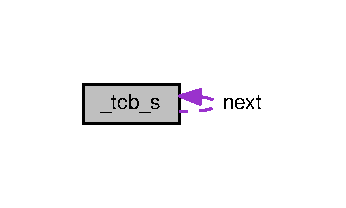
\includegraphics[width=174pt]{struct__tcb__s__coll__graph}
\end{center}
\end{figure}
\subsection*{Data Fields}
\begin{DoxyCompactItemize}
\item 
long $\ast$ {\bfseries sp}\hypertarget{struct__tcb__s_a13f117347df648dbca66e6cbb97a4e0f}{}\label{struct__tcb__s_a13f117347df648dbca66e6cbb97a4e0f}

\item 
struct \hyperlink{struct__tcb__s}{\+\_\+tcb\+\_\+s} $\ast$ {\bfseries next}\hypertarget{struct__tcb__s_af53c260a7b65e7244f809cda9ebb835f}{}\label{struct__tcb__s_af53c260a7b65e7244f809cda9ebb835f}

\item 
uint32\+\_\+t {\bfseries wake\+\_\+time}\hypertarget{struct__tcb__s_a442099ddd859c3f33981828aeef085fe}{}\label{struct__tcb__s_a442099ddd859c3f33981828aeef085fe}

\item 
unsigned long {\bfseries id}\hypertarget{struct__tcb__s_a48e677e5c96cf412d20854802271b9b4}{}\label{struct__tcb__s_a48e677e5c96cf412d20854802271b9b4}

\item 
uint8\+\_\+t {\bfseries priority}\hypertarget{struct__tcb__s_a319151d52db9a3fb0b3c018bce9fcb4a}{}\label{struct__tcb__s_a319151d52db9a3fb0b3c018bce9fcb4a}

\item 
uint32\+\_\+t {\bfseries period}\hypertarget{struct__tcb__s_a85c4e73f3d5ccebf43c628d9e1fc4e4f}{}\label{struct__tcb__s_a85c4e73f3d5ccebf43c628d9e1fc4e4f}

\item 
unsigned long \hyperlink{struct__tcb__s_a1f71cc7a8b23ee420548662caced5301}{magic}\hypertarget{struct__tcb__s_a1f71cc7a8b23ee420548662caced5301}{}\label{struct__tcb__s_a1f71cc7a8b23ee420548662caced5301}

\begin{DoxyCompactList}\small\item\em magic field must contain T\+C\+B\+\_\+\+M\+A\+G\+IC for T\+CB to be valid \end{DoxyCompactList}\item 
void($\ast$ {\bfseries task} )(void)\hypertarget{struct__tcb__s_af815dde5661c4092abe9838fb28d9ed2}{}\label{struct__tcb__s_af815dde5661c4092abe9838fb28d9ed2}

\item 
char $\ast$ {\bfseries task\+\_\+name}\hypertarget{struct__tcb__s_a66241e192445da72f98da4e2d1359d5a}{}\label{struct__tcb__s_a66241e192445da72f98da4e2d1359d5a}

\item 
\hyperlink{struct__pcb__s}{pcb\+\_\+t} $\ast$ {\bfseries parent\+\_\+process}\hypertarget{struct__tcb__s_a95f1ceb9227ec81f5fee8d419e38f6f5}{}\label{struct__tcb__s_a95f1ceb9227ec81f5fee8d419e38f6f5}

\end{DoxyCompactItemize}


The documentation for this struct was generated from the following file\+:\begin{DoxyCompactItemize}
\item 
inc/\hyperlink{OS_8h}{O\+S.\+h}\end{DoxyCompactItemize}

\hypertarget{structevent__t}{}\section{event\+\_\+t Struct Reference}
\label{structevent__t}\index{event\+\_\+t@{event\+\_\+t}}
\subsection*{Data Fields}
\begin{DoxyCompactItemize}
\item 
event\+\_\+type\+\_\+e {\bfseries type}\hypertarget{structevent__t_a9de80e7379b7765ce1be94f1afdbe299}{}\label{structevent__t_a9de80e7379b7765ce1be94f1afdbe299}

\item 
int {\bfseries magic}\hypertarget{structevent__t_a49228cb7c7840507a14a62231e262ed0}{}\label{structevent__t_a49228cb7c7840507a14a62231e262ed0}

\item 
char $\ast$ {\bfseries name}\hypertarget{structevent__t_a5e267e72cb1799268e9333ed5f05dd85}{}\label{structevent__t_a5e267e72cb1799268e9333ed5f05dd85}

\item 
unsigned long long {\bfseries timestamp}\hypertarget{structevent__t_a0597eb180983129aeddc1033f122b5ce}{}\label{structevent__t_a0597eb180983129aeddc1033f122b5ce}

\end{DoxyCompactItemize}


The documentation for this struct was generated from the following file\+:\begin{DoxyCompactItemize}
\item 
inc/\hyperlink{profiler_8h}{profiler.\+h}\end{DoxyCompactItemize}

\hypertarget{structSema4}{}\section{Sema4 Struct Reference}
\label{structSema4}\index{Sema4@{Sema4}}


Collaboration diagram for Sema4\+:\nopagebreak
\begin{figure}[H]
\begin{center}
\leavevmode
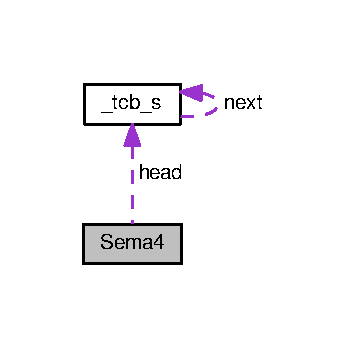
\includegraphics[width=167pt]{structSema4__coll__graph}
\end{center}
\end{figure}
\subsection*{Data Fields}
\begin{DoxyCompactItemize}
\item 
long {\bfseries Value}\hypertarget{structSema4_a98b1e5b4f3a76692bb37db553c22e8b0}{}\label{structSema4_a98b1e5b4f3a76692bb37db553c22e8b0}

\item 
struct \hyperlink{struct__tcb__s}{\+\_\+tcb\+\_\+s} $\ast$ {\bfseries head}\hypertarget{structSema4_a03d774cbfedb9d522f31ded4c10d5668}{}\label{structSema4_a03d774cbfedb9d522f31ded4c10d5668}

\end{DoxyCompactItemize}


The documentation for this struct was generated from the following file\+:\begin{DoxyCompactItemize}
\item 
inc/\hyperlink{OS_8h}{O\+S.\+h}\end{DoxyCompactItemize}

\chapter{File Documentation}
\hypertarget{ADC_8h}{}\section{inc/\+A\+DC.h File Reference}
\label{ADC_8h}\index{inc/\+A\+D\+C.\+h@{inc/\+A\+D\+C.\+h}}


A\+DC driver for the T\+M4\+C123G. Provides interfaces for collecting single samples or a series at a given sampling frequency. Does not allow for sampling of more than one channel at any given time. Timer 2 is reserved for this driver.  


{\ttfamily \#include $<$stdint.\+h$>$}\\*
Include dependency graph for A\+D\+C.\+h\+:\nopagebreak
\begin{figure}[H]
\begin{center}
\leavevmode
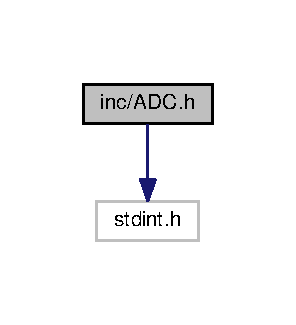
\includegraphics[width=142pt]{ADC_8h__incl}
\end{center}
\end{figure}
\subsection*{Functions}
\begin{DoxyCompactItemize}
\item 
int \hyperlink{ADC_8h_af9d370fc407dee15db32335255f6cf74}{A\+D\+C\+\_\+\+Init} (uint32\+\_\+t channel\+Num)
\begin{DoxyCompactList}\small\item\em Configure an A\+DC channel for continuous sampling. Retrieve measurements from this channel with \hyperlink{ADC_8h_a25269c67b0ba9dd124734e05ffb38493}{A\+D\+C\+\_\+\+In()}. \end{DoxyCompactList}\item 
uint16\+\_\+t \hyperlink{ADC_8h_a25269c67b0ba9dd124734e05ffb38493}{A\+D\+C\+\_\+\+In} (void)
\begin{DoxyCompactList}\small\item\em Returns the most recent sample collected by the channel configured in A\+D\+C\+\_\+\+Init(...) \end{DoxyCompactList}\item 
int \hyperlink{ADC_8h_a262f417393c62f81b4a37b3019b32095}{A\+D\+C\+\_\+\+Collect} (uint32\+\_\+t channel\+Num, uint32\+\_\+t fs, void($\ast$handler)(unsigned long))
\begin{DoxyCompactList}\small\item\em Kick off collection of a sequence of samples to be passed to a user-\/provided handler. The A\+DC and Timer will be configured to collect samples at frequency fs. \end{DoxyCompactList}\end{DoxyCompactItemize}


\subsection{Detailed Description}
A\+DC driver for the T\+M4\+C123G. Provides interfaces for collecting single samples or a series at a given sampling frequency. Does not allow for sampling of more than one channel at any given time. Timer 2 is reserved for this driver. 

\begin{DoxyAuthor}{Author}
Riley Wood and Jeageun Jung 
\end{DoxyAuthor}


\subsection{Function Documentation}
\index{A\+D\+C.\+h@{A\+D\+C.\+h}!A\+D\+C\+\_\+\+Collect@{A\+D\+C\+\_\+\+Collect}}
\index{A\+D\+C\+\_\+\+Collect@{A\+D\+C\+\_\+\+Collect}!A\+D\+C.\+h@{A\+D\+C.\+h}}
\subsubsection[{\texorpdfstring{A\+D\+C\+\_\+\+Collect(uint32\+\_\+t channel\+Num, uint32\+\_\+t fs, void($\ast$handler)(unsigned long))}{ADC_Collect(uint32_t channelNum, uint32_t fs, void(*handler)(unsigned long))}}]{\setlength{\rightskip}{0pt plus 5cm}int A\+D\+C\+\_\+\+Collect (
\begin{DoxyParamCaption}
\item[{uint32\+\_\+t}]{channel\+Num, }
\item[{uint32\+\_\+t}]{fs, }
\item[{void($\ast$)(unsigned long)}]{handler}
\end{DoxyParamCaption}
)}\hypertarget{ADC_8h_a262f417393c62f81b4a37b3019b32095}{}\label{ADC_8h_a262f417393c62f81b4a37b3019b32095}


Kick off collection of a sequence of samples to be passed to a user-\/provided handler. The A\+DC and Timer will be configured to collect samples at frequency fs. 


\begin{DoxyParams}{Parameters}
{\em channel\+Num} & A\+DC channel to sample \\
\hline
{\em fs} & Sampling frequency \\
\hline
{\em handler} & Function which will be passed each sample as it is collected. \\
\hline
\end{DoxyParams}
\begin{DoxyReturn}{Returns}
int 0 on success, -\/1 on failure. 
\end{DoxyReturn}
\index{A\+D\+C.\+h@{A\+D\+C.\+h}!A\+D\+C\+\_\+\+In@{A\+D\+C\+\_\+\+In}}
\index{A\+D\+C\+\_\+\+In@{A\+D\+C\+\_\+\+In}!A\+D\+C.\+h@{A\+D\+C.\+h}}
\subsubsection[{\texorpdfstring{A\+D\+C\+\_\+\+In(void)}{ADC_In(void)}}]{\setlength{\rightskip}{0pt plus 5cm}uint16\+\_\+t A\+D\+C\+\_\+\+In (
\begin{DoxyParamCaption}
\item[{void}]{}
\end{DoxyParamCaption}
)}\hypertarget{ADC_8h_a25269c67b0ba9dd124734e05ffb38493}{}\label{ADC_8h_a25269c67b0ba9dd124734e05ffb38493}


Returns the most recent sample collected by the channel configured in A\+D\+C\+\_\+\+Init(...) 

If the channel has not finished collecting its first sample, this function returns 0x\+F\+F\+FF.

If you call this rapidly, faster than the A\+DC samples, this function may repeat values (since it always returns the most recent).

\begin{DoxyReturn}{Returns}
uint16\+\_\+t The conversion result 
\end{DoxyReturn}
\index{A\+D\+C.\+h@{A\+D\+C.\+h}!A\+D\+C\+\_\+\+Init@{A\+D\+C\+\_\+\+Init}}
\index{A\+D\+C\+\_\+\+Init@{A\+D\+C\+\_\+\+Init}!A\+D\+C.\+h@{A\+D\+C.\+h}}
\subsubsection[{\texorpdfstring{A\+D\+C\+\_\+\+Init(uint32\+\_\+t channel\+Num)}{ADC_Init(uint32_t channelNum)}}]{\setlength{\rightskip}{0pt plus 5cm}int A\+D\+C\+\_\+\+Init (
\begin{DoxyParamCaption}
\item[{uint32\+\_\+t}]{channel\+Num}
\end{DoxyParamCaption}
)}\hypertarget{ADC_8h_af9d370fc407dee15db32335255f6cf74}{}\label{ADC_8h_af9d370fc407dee15db32335255f6cf74}


Configure an A\+DC channel for continuous sampling. Retrieve measurements from this channel with \hyperlink{ADC_8h_a25269c67b0ba9dd124734e05ffb38493}{A\+D\+C\+\_\+\+In()}. 


\begin{DoxyParams}{Parameters}
{\em channel\+Num} & The channel to set up \\
\hline
\end{DoxyParams}
\begin{DoxyReturn}{Returns}
int 0 on success, -\/1 on failure. 
\end{DoxyReturn}

\hypertarget{interpreter_8h}{}\section{inc/interpreter.h File Reference}
\label{interpreter_8h}\index{inc/interpreter.\+h@{inc/interpreter.\+h}}
\subsection*{Functions}
\begin{DoxyCompactItemize}
\item 
void \hyperlink{interpreter_8h_a0cf6f7b20306bd53e7f61b3ead179154}{interpreter\+\_\+task} (void)\hypertarget{interpreter_8h_a0cf6f7b20306bd53e7f61b3ead179154}{}\label{interpreter_8h_a0cf6f7b20306bd53e7f61b3ead179154}

\begin{DoxyCompactList}\small\item\em OS Task that sends characters to the interpreter. \end{DoxyCompactList}\item 
void \hyperlink{interpreter_8h_ad36afca5c99ec60b995fae704d95d014}{interpreter\+\_\+cmd} (char $\ast$cmd\+\_\+str)
\begin{DoxyCompactList}\small\item\em Pass user input to the interpreter and act on their command. \end{DoxyCompactList}\end{DoxyCompactItemize}


\subsection{Detailed Description}
List of commands
\begin{DoxyItemize}
\item adc
\begin{DoxyItemize}
\item Prints 2 consecutive A\+DC samples of channel 0 to the L\+CD and U\+A\+R\+T0
\end{DoxyItemize}
\item lcd
\begin{DoxyItemize}
\item Prints strings on each line of each logical display on the L\+CD.
\end{DoxyItemize}
\item critical
\begin{DoxyItemize}
\item Prints the percentage of C\+PU time spent with interrupts disabled.
\end{DoxyItemize}
\item log
\begin{DoxyItemize}
\item Prints profiler events logged
\end{DoxyItemize}
\item clear
\begin{DoxyItemize}
\item Clears the profiler event log and restarts the profiler
\end{DoxyItemize}
\item format
\begin{DoxyItemize}
\item Formats the filesystem on the SD card
\end{DoxyItemize}
\item ls
\begin{DoxyItemize}
\item List all files in the filesystem
\end{DoxyItemize}
\item cat
\begin{DoxyItemize}
\item Print out file in the filesystem.
\item Takes one argument\+: the name of the file to print
\end{DoxyItemize}
\item rm
\begin{DoxyItemize}
\item Remove file in the filesystem.
\item Takes one argument\+: the name of the file to remove
\end{DoxyItemize}
\item touch
\begin{DoxyItemize}
\item Create a file in the filesystem.
\item Takes one argument\+: the name of the file to create
\end{DoxyItemize}
\item echo
\begin{DoxyItemize}
\item Append characters to a file
\item Takes two arguments in this order\+:
\begin{DoxyItemize}
\item The name of the file to append to
\item Remaining characters are written to the file
\end{DoxyItemize}
\end{DoxyItemize}
\item increase
\begin{DoxyItemize}
\item Artificially increase the time spent in critical sections to test the \char`\"{}critical\char`\"{} command. 
\end{DoxyItemize}
\end{DoxyItemize}

\subsection{Function Documentation}
\index{interpreter.\+h@{interpreter.\+h}!interpreter\+\_\+cmd@{interpreter\+\_\+cmd}}
\index{interpreter\+\_\+cmd@{interpreter\+\_\+cmd}!interpreter.\+h@{interpreter.\+h}}
\subsubsection[{\texorpdfstring{interpreter\+\_\+cmd(char $\ast$cmd\+\_\+str)}{interpreter_cmd(char *cmd_str)}}]{\setlength{\rightskip}{0pt plus 5cm}void interpreter\+\_\+cmd (
\begin{DoxyParamCaption}
\item[{char $\ast$}]{cmd\+\_\+str}
\end{DoxyParamCaption}
)}\hypertarget{interpreter_8h_ad36afca5c99ec60b995fae704d95d014}{}\label{interpreter_8h_ad36afca5c99ec60b995fae704d95d014}


Pass user input to the interpreter and act on their command. 


\begin{DoxyParams}{Parameters}
{\em cmd\+\_\+str} & String containing the entire user command. \\
\hline
\end{DoxyParams}

\hypertarget{misc__macros_8h}{}\section{inc/misc\+\_\+macros.h File Reference}
\label{misc__macros_8h}\index{inc/misc\+\_\+macros.\+h@{inc/misc\+\_\+macros.\+h}}


Some helper macros.  


\subsection*{Macros}
\begin{DoxyCompactItemize}
\item 
\#define \hyperlink{misc__macros_8h_ad53b2827d15d4f100433764eea395a94}{lengthof}(array)~(sizeof(array)/sizeof((array)\mbox{[}0\mbox{]}))\hypertarget{misc__macros_8h_ad53b2827d15d4f100433764eea395a94}{}\label{misc__macros_8h_ad53b2827d15d4f100433764eea395a94}

\begin{DoxyCompactList}\small\item\em Get the number of elements in an array. \end{DoxyCompactList}\item 
\#define \hyperlink{misc__macros_8h_a06311b356862bfe3ac93fedc89c5c066}{zeroes}(array)~memset(array, 0, sizeof(array))\hypertarget{misc__macros_8h_a06311b356862bfe3ac93fedc89c5c066}{}\label{misc__macros_8h_a06311b356862bfe3ac93fedc89c5c066}

\begin{DoxyCompactList}\small\item\em Zeroes out an array. \end{DoxyCompactList}\end{DoxyCompactItemize}


\subsection{Detailed Description}
Some helper macros. 


\hypertarget{OS_8h}{}\section{inc/\+OS.h File Reference}
\label{OS_8h}\index{inc/\+O\+S.\+h@{inc/\+O\+S.\+h}}


Real Time Operating System for Labs 2 and 3 E\+E445\+M/\+E\+E380\+L.\+12.  


{\ttfamily \#include $<$stdint.\+h$>$}\\*
Include dependency graph for O\+S.\+h\+:\nopagebreak
\begin{figure}[H]
\begin{center}
\leavevmode
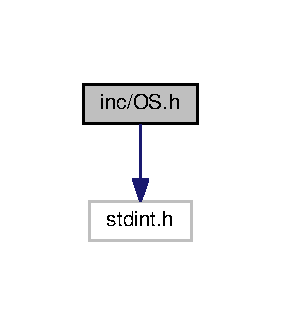
\includegraphics[width=135pt]{OS_8h__incl}
\end{center}
\end{figure}
This graph shows which files directly or indirectly include this file\+:\nopagebreak
\begin{figure}[H]
\begin{center}
\leavevmode
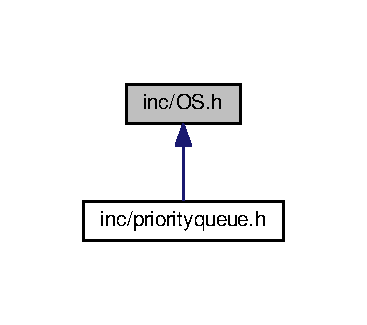
\includegraphics[width=176pt]{OS_8h__dep__incl}
\end{center}
\end{figure}
\subsection*{Data Structures}
\begin{DoxyCompactItemize}
\item 
struct \hyperlink{struct__pcb__s}{\+\_\+pcb\+\_\+s}
\item 
struct \hyperlink{struct__tcb__s}{\+\_\+tcb\+\_\+s}
\item 
struct \hyperlink{structSema4}{Sema4}
\end{DoxyCompactItemize}
\subsection*{Macros}
\begin{DoxyCompactItemize}
\item 
\#define {\bfseries T\+I\+M\+E\+\_\+1\+MS}~80000\hypertarget{OS_8h_ad6445469b3084b0c8a8ea272e8a40a17}{}\label{OS_8h_ad6445469b3084b0c8a8ea272e8a40a17}

\item 
\#define {\bfseries T\+I\+M\+E\+\_\+2\+MS}~(2 $\ast$ T\+I\+M\+E\+\_\+1\+MS)\hypertarget{OS_8h_a601fb0d91385070bae69c2b1c4e63162}{}\label{OS_8h_a601fb0d91385070bae69c2b1c4e63162}

\item 
\#define {\bfseries T\+I\+M\+E\+\_\+500\+US}~(T\+I\+M\+E\+\_\+1\+MS / 2)\hypertarget{OS_8h_a5bd8a6024a3e7cd43b7fe30988ca81e8}{}\label{OS_8h_a5bd8a6024a3e7cd43b7fe30988ca81e8}

\item 
\#define {\bfseries T\+I\+M\+E\+\_\+250\+US}~(T\+I\+M\+E\+\_\+1\+MS / 4)\hypertarget{OS_8h_aae4936d8a1bad649da44cacada40b157}{}\label{OS_8h_aae4936d8a1bad649da44cacada40b157}

\item 
\#define {\bfseries T\+A\+S\+K\+\_\+\+S\+T\+A\+C\+K\+\_\+\+S\+I\+ZE}~128\hypertarget{OS_8h_a5486258f1f34d3baeda92a74b63c27c3}{}\label{OS_8h_a5486258f1f34d3baeda92a74b63c27c3}

\item 
\#define {\bfseries T\+C\+B\+\_\+\+M\+A\+G\+IC}~(0x900d900d)\hypertarget{OS_8h_a0fb8aa2f0ea0a6494f1639dd97087013}{}\label{OS_8h_a0fb8aa2f0ea0a6494f1639dd97087013}

\item 
\#define \hyperlink{OS_8h_accb79b9446dd2b953a1fb8437c5f6e15}{O\+S\+\_\+\+Add\+Thread}(task,  stack\+Size,  priority)
\item 
\#define \hyperlink{OS_8h_adf56561acbee98b34e8c42ff6b147255}{O\+S\+\_\+\+Add\+Periodic\+Thread}(task,  period,  priority)~O\+S\+\_\+\+Add\+Periodic\+Thread\+\_\+priv(task, period, priority, \#task)
\end{DoxyCompactItemize}
\subsection*{Typedefs}
\begin{DoxyCompactItemize}
\item 
typedef struct \hyperlink{struct__pcb__s}{\+\_\+pcb\+\_\+s} {\bfseries pcb\+\_\+t}\hypertarget{OS_8h_add17966847109f7551977a87ddfcd8aa}{}\label{OS_8h_add17966847109f7551977a87ddfcd8aa}

\item 
typedef struct \hyperlink{struct__tcb__s}{\+\_\+tcb\+\_\+s} {\bfseries tcb\+\_\+t}\hypertarget{OS_8h_a5f5b511a2a589828581399459da62c6a}{}\label{OS_8h_a5f5b511a2a589828581399459da62c6a}

\item 
typedef struct \hyperlink{structSema4}{Sema4} {\bfseries Sema4\+Type}\hypertarget{OS_8h_a798fbe37dbc49a5ff9af51bf7de1ee8e}{}\label{OS_8h_a798fbe37dbc49a5ff9af51bf7de1ee8e}

\end{DoxyCompactItemize}
\subsection*{Functions}
\begin{DoxyCompactItemize}
\item 
void \hyperlink{OS_8h_acb6df8f47f418aad9c9a9e045d7d1e6d}{O\+S\+\_\+\+Init} (void)
\item 
void \hyperlink{OS_8h_af580c6222330cc3d214763ddac7800b9}{O\+S\+\_\+\+Init\+Semaphore} (\hyperlink{structSema4}{Sema4\+Type} $\ast$sema\+Pt, long value)
\item 
void \hyperlink{OS_8h_aad29612829941c857ed685f40e193cd0}{O\+S\+\_\+\+Wait} (\hyperlink{structSema4}{Sema4\+Type} $\ast$sema\+Pt)
\item 
void \hyperlink{OS_8h_a0c4d587c411a23652529110910261fde}{O\+S\+\_\+\+Signal} (\hyperlink{structSema4}{Sema4\+Type} $\ast$sema\+Pt)
\item 
void \hyperlink{OS_8h_a3f127f7a40ffd3e43b7b0f4c8b7f30ff}{O\+S\+\_\+b\+Wait} (\hyperlink{structSema4}{Sema4\+Type} $\ast$sema\+Pt)
\item 
void \hyperlink{OS_8h_aacf0c377b570fc63b103c57e0fbc7acd}{O\+S\+\_\+b\+Signal} (\hyperlink{structSema4}{Sema4\+Type} $\ast$sema\+Pt)
\item 
void \hyperlink{OS_8h_a075cf7301361417f66be1d5c22e36b0f}{Jitter} (void)\hypertarget{OS_8h_a075cf7301361417f66be1d5c22e36b0f}{}\label{OS_8h_a075cf7301361417f66be1d5c22e36b0f}

\begin{DoxyCompactList}\small\item\em Print the max periodic task jitter measured thus far to the S\+T7735 display. \end{DoxyCompactList}\item 
int {\bfseries \+\_\+\+\_\+\+O\+S\+\_\+\+Add\+Thread} (void($\ast$task)(void), unsigned long stack\+Size, unsigned long priority, char $\ast$task\+\_\+name, \hyperlink{struct__pcb__s}{pcb\+\_\+t} $\ast$parent\+\_\+process)\hypertarget{OS_8h_a3e5c42edf8d08a40ccdee09e200d84b6}{}\label{OS_8h_a3e5c42edf8d08a40ccdee09e200d84b6}

\item 
unsigned long \hyperlink{OS_8h_adc21b8aab03cbb1611186ca3ac9123d8}{O\+S\+\_\+\+Id} (void)
\item 
int {\bfseries O\+S\+\_\+\+Add\+Periodic\+Thread\+\_\+priv} (void($\ast$task)(void), unsigned long period, unsigned long priority, char $\ast$task\+\_\+name)\hypertarget{OS_8h_a21ee017683a4a2b593d5497a27addac0}{}\label{OS_8h_a21ee017683a4a2b593d5497a27addac0}

\item 
int \hyperlink{OS_8h_a5c387e683842fc4f9f846729a60186da}{O\+S\+\_\+\+Add\+S\+W1\+Task} (void($\ast$task)(void), unsigned long priority)
\item 
int \hyperlink{OS_8h_a508ed7f6202df8a9e500994ad4399784}{O\+S\+\_\+\+Add\+S\+W2\+Task} (void($\ast$task)(void), unsigned long priority)
\item 
void \hyperlink{OS_8h_aeeb2aca9e1a16738a5d82353b2d497ac}{O\+S\+\_\+\+Sleep} (unsigned long sleep\+Time)
\item 
void \hyperlink{OS_8h_a8e991f4f2576c5cfec04ef5f37aabea5}{O\+S\+\_\+\+Kill} (void)
\item 
void \hyperlink{OS_8h_a4e71587568a2a48931a35615cad1b5db}{O\+S\+\_\+\+Suspend} (void)
\item 
void \hyperlink{OS_8h_a361ff1137f5dad8e0a74631be6fb12b6}{O\+S\+\_\+\+Fifo\+\_\+\+Init} (unsigned long size)
\item 
int \hyperlink{OS_8h_adf231073602c9328f6248f6272d63e7f}{O\+S\+\_\+\+Fifo\+\_\+\+Put} (unsigned long data)
\item 
unsigned long \hyperlink{OS_8h_af899a42296039e22ffdd8bf6e1ca208e}{O\+S\+\_\+\+Fifo\+\_\+\+Get} (void)
\item 
long \hyperlink{OS_8h_a9ff4cb899801f20ff90cbf2717c154c7}{O\+S\+\_\+\+Fifo\+\_\+\+Size} (void)
\item 
void \hyperlink{OS_8h_a84e1a933dd73e319fdd5649c2270281b}{O\+S\+\_\+\+Mail\+Box\+\_\+\+Init} (void)
\item 
void \hyperlink{OS_8h_ac4c3ebdb61c0c11195d6fcafeb0d4c99}{O\+S\+\_\+\+Mail\+Box\+\_\+\+Send} (unsigned long data)
\item 
unsigned long \hyperlink{OS_8h_ace71083584f0f1e5e2f081f1e4a1394a}{O\+S\+\_\+\+Mail\+Box\+\_\+\+Recv} (void)
\item 
unsigned long long \hyperlink{OS_8h_a5798d7fa05a4c3a523efe1b5651c5318}{O\+S\+\_\+\+Time} (void)
\item 
unsigned long long \hyperlink{OS_8h_af4b27f93116607bd3986125cb1c9edcf}{O\+S\+\_\+\+Time\+Difference} (unsigned long long start, unsigned long long stop)
\item 
void \hyperlink{OS_8h_ace6ec4b7947542f7d7ff3104d8c759bd}{O\+S\+\_\+\+Clear\+Ms\+Time} (void)
\item 
unsigned long \hyperlink{OS_8h_a251073790d2782617fd7474625761573}{O\+S\+\_\+\+Ms\+Time} (void)
\item 
void \hyperlink{OS_8h_a18553a7e1d82dcaaeb80a5524bd01cf2}{O\+S\+\_\+\+Launch} (unsigned long the\+Time\+Slice)
\item 
int \hyperlink{OS_8h_a3271236396a143a19c9650377e0f32ee}{O\+S\+\_\+\+Add\+Process} (void($\ast$entry)(void), void $\ast$text, void $\ast$data, unsigned long stack\+Size, unsigned long priority)
\begin{DoxyCompactList}\small\item\em Launch a process in the OS. \end{DoxyCompactList}\item 
long {\bfseries Start\+Critical} (void)\hypertarget{OS_8h_a6e7e2088607214bc15b17ac57b57df1b}{}\label{OS_8h_a6e7e2088607214bc15b17ac57b57df1b}

\item 
void {\bfseries End\+Critical} (long sr)\hypertarget{OS_8h_a670da3ff1aea0c7d54c40e9e40b5eeed}{}\label{OS_8h_a670da3ff1aea0c7d54c40e9e40b5eeed}

\item 
void {\bfseries Disable\+Interrupts} (void)\hypertarget{OS_8h_ac866dbaf7b167e5c46bb33de42eee84d}{}\label{OS_8h_ac866dbaf7b167e5c46bb33de42eee84d}

\item 
void {\bfseries Enable\+Interrupts} (void)\hypertarget{OS_8h_ab712356331a62b04aebcb373865e68c4}{}\label{OS_8h_ab712356331a62b04aebcb373865e68c4}

\end{DoxyCompactItemize}
\subsection*{Variables}
\begin{DoxyCompactItemize}
\item 
\hyperlink{struct__tcb__s}{tcb\+\_\+t} $\ast$ {\bfseries cur\+\_\+tcb}\hypertarget{OS_8h_aa1c72d659051f84119a2c6373fe43bee}{}\label{OS_8h_aa1c72d659051f84119a2c6373fe43bee}

\end{DoxyCompactItemize}


\subsection{Detailed Description}
Real Time Operating System for Labs 2 and 3 E\+E445\+M/\+E\+E380\+L.\+12. 

R\+T\+OS kernel capable of round-\/robin scheduling, up to 2 low-\/jitter periodic tasks.

Reserves W\+T\+I\+M\+E\+R1A and B for periodic task scheduling. Reserves Sys\+Tick timer for round-\/robin scheduling. Reserves W\+T\+I\+M\+E\+R0 as a 64-\/bit time source.

Interface by Jonathan W. Valvano 2/20/17, \href{mailto:valvano@mail.utexas.edu}{\tt valvano@mail.\+utexas.\+edu} Implementation by Riley Wood and Jeageun Jung \begin{DoxyAuthor}{Author}
Riley Wood and Jeageun Jung 
\end{DoxyAuthor}


\subsection{Macro Definition Documentation}
\index{O\+S.\+h@{O\+S.\+h}!O\+S\+\_\+\+Add\+Periodic\+Thread@{O\+S\+\_\+\+Add\+Periodic\+Thread}}
\index{O\+S\+\_\+\+Add\+Periodic\+Thread@{O\+S\+\_\+\+Add\+Periodic\+Thread}!O\+S.\+h@{O\+S.\+h}}
\subsubsection[{\texorpdfstring{O\+S\+\_\+\+Add\+Periodic\+Thread}{OS_AddPeriodicThread}}]{\setlength{\rightskip}{0pt plus 5cm}\#define O\+S\+\_\+\+Add\+Periodic\+Thread(
\begin{DoxyParamCaption}
\item[{}]{task, }
\item[{}]{period, }
\item[{}]{priority}
\end{DoxyParamCaption}
)~O\+S\+\_\+\+Add\+Periodic\+Thread\+\_\+priv(task, period, priority, \#task)}\hypertarget{OS_8h_adf56561acbee98b34e8c42ff6b147255}{}\label{OS_8h_adf56561acbee98b34e8c42ff6b147255}
Add a background periodic task. Typically this function receives the highest priority You are free to select the time resolution for this function It is assumed that the user task will run to completion and return This task can not spin, block, loop, sleep, or kill This task can call O\+S\+\_\+\+Signal O\+S\+\_\+b\+Signal O\+S\+\_\+\+Add\+Thread This task does not have a Thread ID In lab 2, this command will be called 0 or 1 times In lab 2, the priority field can be ignored In lab 3, this command will be called 0 1 or 2 times In lab 3, there will be up to four background threads, and this priority field determines the relative priority of these four threads 
\begin{DoxyParams}{Parameters}
{\em task} & pointer to a void/void background function \\
\hline
{\em period} & given in system time units (12.\+5ns) \\
\hline
{\em priority} & 0 is the highest, 5 is the lowest \\
\hline
\end{DoxyParams}
\begin{DoxyReturn}{Returns}
1 if successful, 0 if this thread can not be added 
\end{DoxyReturn}
\index{O\+S.\+h@{O\+S.\+h}!O\+S\+\_\+\+Add\+Thread@{O\+S\+\_\+\+Add\+Thread}}
\index{O\+S\+\_\+\+Add\+Thread@{O\+S\+\_\+\+Add\+Thread}!O\+S.\+h@{O\+S.\+h}}
\subsubsection[{\texorpdfstring{O\+S\+\_\+\+Add\+Thread}{OS_AddThread}}]{\setlength{\rightskip}{0pt plus 5cm}\#define O\+S\+\_\+\+Add\+Thread(
\begin{DoxyParamCaption}
\item[{}]{task, }
\item[{}]{stack\+Size, }
\item[{}]{priority}
\end{DoxyParamCaption}
)}\hypertarget{OS_8h_accb79b9446dd2b953a1fb8437c5f6e15}{}\label{OS_8h_accb79b9446dd2b953a1fb8437c5f6e15}
{\bfseries Value\+:}
\begin{DoxyCode}
\_\_OS\_AddThread(task,\(\backslash\)
                                                               stackSize,\(\backslash\)
                                                               priority,\(\backslash\)
                                                               #task,\(\backslash\)
                                                               cur\_tcb ? cur\_tcb->parent\_process : 0)
\end{DoxyCode}
add a foregound thread to the scheduler stack size must be divisable by 8 (aligned to double word boundary) In Lab 2, you can ignore both the stack\+Size and priority fields In Lab 3, you can ignore the stack\+Size fields 
\begin{DoxyParams}{Parameters}
{\em task} & Task function \\
\hline
{\em stack\+Size} & Size of the stack in bytes. Should be divisible by 8 \\
\hline
{\em priority} & Priority of the task. 0 is highest, 5 is lowest. \\
\hline
\end{DoxyParams}
\begin{DoxyReturn}{Returns}
1 if successful, 0 if this thread can not be added 
\end{DoxyReturn}


\subsection{Function Documentation}
\index{O\+S.\+h@{O\+S.\+h}!O\+S\+\_\+\+Add\+Process@{O\+S\+\_\+\+Add\+Process}}
\index{O\+S\+\_\+\+Add\+Process@{O\+S\+\_\+\+Add\+Process}!O\+S.\+h@{O\+S.\+h}}
\subsubsection[{\texorpdfstring{O\+S\+\_\+\+Add\+Process(void($\ast$entry)(void), void $\ast$text, void $\ast$data, unsigned long stack\+Size, unsigned long priority)}{OS_AddProcess(void(*entry)(void), void *text, void *data, unsigned long stackSize, unsigned long priority)}}]{\setlength{\rightskip}{0pt plus 5cm}int O\+S\+\_\+\+Add\+Process (
\begin{DoxyParamCaption}
\item[{void($\ast$)(void)}]{entry, }
\item[{void $\ast$}]{text, }
\item[{void $\ast$}]{data, }
\item[{unsigned long}]{stack\+Size, }
\item[{unsigned long}]{priority}
\end{DoxyParamCaption}
)}\hypertarget{OS_8h_a3271236396a143a19c9650377e0f32ee}{}\label{OS_8h_a3271236396a143a19c9650377e0f32ee}


Launch a process in the OS. 


\begin{DoxyParams}{Parameters}
{\em entry} & Entry point, usually main() of the process \\
\hline
{\em text} & Text (code) section start address \\
\hline
{\em data} & Data section start address \\
\hline
{\em stack\+Size} & Size of the stack for the first thread \\
\hline
{\em priority} & Priority for the first thread \\
\hline
\end{DoxyParams}
\begin{DoxyReturn}{Returns}
int 0 on success, -\/1 on failure. 
\end{DoxyReturn}
\index{O\+S.\+h@{O\+S.\+h}!O\+S\+\_\+\+Add\+S\+W1\+Task@{O\+S\+\_\+\+Add\+S\+W1\+Task}}
\index{O\+S\+\_\+\+Add\+S\+W1\+Task@{O\+S\+\_\+\+Add\+S\+W1\+Task}!O\+S.\+h@{O\+S.\+h}}
\subsubsection[{\texorpdfstring{O\+S\+\_\+\+Add\+S\+W1\+Task(void($\ast$task)(void), unsigned long priority)}{OS_AddSW1Task(void(*task)(void), unsigned long priority)}}]{\setlength{\rightskip}{0pt plus 5cm}int O\+S\+\_\+\+Add\+S\+W1\+Task (
\begin{DoxyParamCaption}
\item[{void($\ast$)(void)}]{task, }
\item[{unsigned long}]{priority}
\end{DoxyParamCaption}
)}\hypertarget{OS_8h_a5c387e683842fc4f9f846729a60186da}{}\label{OS_8h_a5c387e683842fc4f9f846729a60186da}
add a background task to run whenever the S\+W1 (P\+F4) button is pushed 
\begin{DoxyParams}{Parameters}
{\em pointer} & to a void/void background function \\
\hline
{\em priority} & 0 is the highest, 5 is the lowest \\
\hline
\end{DoxyParams}
\begin{DoxyReturn}{Returns}
1 if successful, 0 if this thread can not be added It is assumed that the user task will run to completion and return This task can not spin, block, loop, sleep, or kill This task can call O\+S\+\_\+\+Signal O\+S\+\_\+b\+Signal O\+S\+\_\+\+Add\+Thread This task does not have a Thread ID In labs 2 and 3, this command will be called 0 or 1 times In lab 2, the priority field can be ignored In lab 3, there will be up to four background threads, and this priority field determines the relative priority of these four threads 
\end{DoxyReturn}
\index{O\+S.\+h@{O\+S.\+h}!O\+S\+\_\+\+Add\+S\+W2\+Task@{O\+S\+\_\+\+Add\+S\+W2\+Task}}
\index{O\+S\+\_\+\+Add\+S\+W2\+Task@{O\+S\+\_\+\+Add\+S\+W2\+Task}!O\+S.\+h@{O\+S.\+h}}
\subsubsection[{\texorpdfstring{O\+S\+\_\+\+Add\+S\+W2\+Task(void($\ast$task)(void), unsigned long priority)}{OS_AddSW2Task(void(*task)(void), unsigned long priority)}}]{\setlength{\rightskip}{0pt plus 5cm}int O\+S\+\_\+\+Add\+S\+W2\+Task (
\begin{DoxyParamCaption}
\item[{void($\ast$)(void)}]{task, }
\item[{unsigned long}]{priority}
\end{DoxyParamCaption}
)}\hypertarget{OS_8h_a508ed7f6202df8a9e500994ad4399784}{}\label{OS_8h_a508ed7f6202df8a9e500994ad4399784}
add a background task to run whenever the S\+W2 (P\+F0) button is pushed 
\begin{DoxyParams}{Parameters}
{\em pointer} & to a void/void background function \\
\hline
{\em priority} & 0 is highest, 5 is lowest \\
\hline
\end{DoxyParams}
\begin{DoxyReturn}{Returns}
1 if successful, 0 if this thread can not be added It is assumed user task will run to completion and return This task can not spin block loop sleep or kill This task can call issue O\+S\+\_\+\+Signal, it can call O\+S\+\_\+\+Add\+Thread This task does not have a Thread ID In lab 2, this function can be ignored In lab 3, this command will be called will be called 0 or 1 times In lab 3, there will be up to four background threads, and this priority field determines the relative priority of these four threads 
\end{DoxyReturn}
\index{O\+S.\+h@{O\+S.\+h}!O\+S\+\_\+b\+Signal@{O\+S\+\_\+b\+Signal}}
\index{O\+S\+\_\+b\+Signal@{O\+S\+\_\+b\+Signal}!O\+S.\+h@{O\+S.\+h}}
\subsubsection[{\texorpdfstring{O\+S\+\_\+b\+Signal(\+Sema4\+Type $\ast$sema\+Pt)}{OS_bSignal(Sema4Type *semaPt)}}]{\setlength{\rightskip}{0pt plus 5cm}void O\+S\+\_\+b\+Signal (
\begin{DoxyParamCaption}
\item[{{\bf Sema4\+Type} $\ast$}]{sema\+Pt}
\end{DoxyParamCaption}
)}\hypertarget{OS_8h_aacf0c377b570fc63b103c57e0fbc7acd}{}\label{OS_8h_aacf0c377b570fc63b103c57e0fbc7acd}
Lab2 spinlock, set to 1 Lab3 wakeup blocked thread if appropriate 
\begin{DoxyParams}{Parameters}
{\em sema\+Pt} & pointer to a binary semaphore \\
\hline
\end{DoxyParams}
\index{O\+S.\+h@{O\+S.\+h}!O\+S\+\_\+b\+Wait@{O\+S\+\_\+b\+Wait}}
\index{O\+S\+\_\+b\+Wait@{O\+S\+\_\+b\+Wait}!O\+S.\+h@{O\+S.\+h}}
\subsubsection[{\texorpdfstring{O\+S\+\_\+b\+Wait(\+Sema4\+Type $\ast$sema\+Pt)}{OS_bWait(Sema4Type *semaPt)}}]{\setlength{\rightskip}{0pt plus 5cm}void O\+S\+\_\+b\+Wait (
\begin{DoxyParamCaption}
\item[{{\bf Sema4\+Type} $\ast$}]{sema\+Pt}
\end{DoxyParamCaption}
)}\hypertarget{OS_8h_a3f127f7a40ffd3e43b7b0f4c8b7f30ff}{}\label{OS_8h_a3f127f7a40ffd3e43b7b0f4c8b7f30ff}
Lab2 spinlock, set to 0 Lab3 block if less than zero 
\begin{DoxyParams}{Parameters}
{\em sema\+Pt} & pointer to a binary semaphore \\
\hline
\end{DoxyParams}
\index{O\+S.\+h@{O\+S.\+h}!O\+S\+\_\+\+Clear\+Ms\+Time@{O\+S\+\_\+\+Clear\+Ms\+Time}}
\index{O\+S\+\_\+\+Clear\+Ms\+Time@{O\+S\+\_\+\+Clear\+Ms\+Time}!O\+S.\+h@{O\+S.\+h}}
\subsubsection[{\texorpdfstring{O\+S\+\_\+\+Clear\+Ms\+Time(void)}{OS_ClearMsTime(void)}}]{\setlength{\rightskip}{0pt plus 5cm}void O\+S\+\_\+\+Clear\+Ms\+Time (
\begin{DoxyParamCaption}
\item[{void}]{}
\end{DoxyParamCaption}
)}\hypertarget{OS_8h_ace6ec4b7947542f7d7ff3104d8c759bd}{}\label{OS_8h_ace6ec4b7947542f7d7ff3104d8c759bd}
Sets the system time to zero (from Lab 1). You are free to change how this works. \begin{DoxyReturn}{Returns}
none 
\end{DoxyReturn}
\index{O\+S.\+h@{O\+S.\+h}!O\+S\+\_\+\+Fifo\+\_\+\+Get@{O\+S\+\_\+\+Fifo\+\_\+\+Get}}
\index{O\+S\+\_\+\+Fifo\+\_\+\+Get@{O\+S\+\_\+\+Fifo\+\_\+\+Get}!O\+S.\+h@{O\+S.\+h}}
\subsubsection[{\texorpdfstring{O\+S\+\_\+\+Fifo\+\_\+\+Get(void)}{OS_Fifo_Get(void)}}]{\setlength{\rightskip}{0pt plus 5cm}unsigned long O\+S\+\_\+\+Fifo\+\_\+\+Get (
\begin{DoxyParamCaption}
\item[{void}]{}
\end{DoxyParamCaption}
)}\hypertarget{OS_8h_af899a42296039e22ffdd8bf6e1ca208e}{}\label{OS_8h_af899a42296039e22ffdd8bf6e1ca208e}
Remove one data sample from the Fifo. Called in foreground, will spin/block if empty \begin{DoxyReturn}{Returns}
data 
\end{DoxyReturn}
\index{O\+S.\+h@{O\+S.\+h}!O\+S\+\_\+\+Fifo\+\_\+\+Init@{O\+S\+\_\+\+Fifo\+\_\+\+Init}}
\index{O\+S\+\_\+\+Fifo\+\_\+\+Init@{O\+S\+\_\+\+Fifo\+\_\+\+Init}!O\+S.\+h@{O\+S.\+h}}
\subsubsection[{\texorpdfstring{O\+S\+\_\+\+Fifo\+\_\+\+Init(unsigned long size)}{OS_Fifo_Init(unsigned long size)}}]{\setlength{\rightskip}{0pt plus 5cm}void O\+S\+\_\+\+Fifo\+\_\+\+Init (
\begin{DoxyParamCaption}
\item[{unsigned long}]{size}
\end{DoxyParamCaption}
)}\hypertarget{OS_8h_a361ff1137f5dad8e0a74631be6fb12b6}{}\label{OS_8h_a361ff1137f5dad8e0a74631be6fb12b6}
Initialize the Fifo to be empty. In Lab 2, you can ignore the size field. In Lab 3, you should implement the user-\/defined fifo size. In Lab 3, you can put whatever restrictions you want on size e.\+g., 4 to 64 elements e.\+g., must be a power of 2,4,8,16,32,64,128 
\begin{DoxyParams}{Parameters}
{\em size} & Size of the fifo \\
\hline
\end{DoxyParams}
\begin{DoxyReturn}{Returns}
none 
\end{DoxyReturn}
\index{O\+S.\+h@{O\+S.\+h}!O\+S\+\_\+\+Fifo\+\_\+\+Put@{O\+S\+\_\+\+Fifo\+\_\+\+Put}}
\index{O\+S\+\_\+\+Fifo\+\_\+\+Put@{O\+S\+\_\+\+Fifo\+\_\+\+Put}!O\+S.\+h@{O\+S.\+h}}
\subsubsection[{\texorpdfstring{O\+S\+\_\+\+Fifo\+\_\+\+Put(unsigned long data)}{OS_Fifo_Put(unsigned long data)}}]{\setlength{\rightskip}{0pt plus 5cm}int O\+S\+\_\+\+Fifo\+\_\+\+Put (
\begin{DoxyParamCaption}
\item[{unsigned long}]{data}
\end{DoxyParamCaption}
)}\hypertarget{OS_8h_adf231073602c9328f6248f6272d63e7f}{}\label{OS_8h_adf231073602c9328f6248f6272d63e7f}
Enter one data sample into the Fifo. Called from the background, so no waiting. Since this is called by interrupt handlers this function can not disable or enable interrupts. 
\begin{DoxyParams}{Parameters}
{\em data} & Data to put in the F\+I\+FO \\
\hline
\end{DoxyParams}
\begin{DoxyReturn}{Returns}
true if data is properly saved, false if data not saved, because it was full 
\end{DoxyReturn}
\index{O\+S.\+h@{O\+S.\+h}!O\+S\+\_\+\+Fifo\+\_\+\+Size@{O\+S\+\_\+\+Fifo\+\_\+\+Size}}
\index{O\+S\+\_\+\+Fifo\+\_\+\+Size@{O\+S\+\_\+\+Fifo\+\_\+\+Size}!O\+S.\+h@{O\+S.\+h}}
\subsubsection[{\texorpdfstring{O\+S\+\_\+\+Fifo\+\_\+\+Size(void)}{OS_Fifo_Size(void)}}]{\setlength{\rightskip}{0pt plus 5cm}long O\+S\+\_\+\+Fifo\+\_\+\+Size (
\begin{DoxyParamCaption}
\item[{void}]{}
\end{DoxyParamCaption}
)}\hypertarget{OS_8h_a9ff4cb899801f20ff90cbf2717c154c7}{}\label{OS_8h_a9ff4cb899801f20ff90cbf2717c154c7}
Check the status of the Fifo. \begin{DoxyReturn}{Returns}
returns the number of elements in the Fifo. Greater than zero if a call to O\+S\+\_\+\+Fifo\+\_\+\+Get will return right away, zero or less than zero if the Fifo is empty, zero or less than zero if a call to O\+S\+\_\+\+Fifo\+\_\+\+Get will spin or block 
\end{DoxyReturn}
\index{O\+S.\+h@{O\+S.\+h}!O\+S\+\_\+\+Id@{O\+S\+\_\+\+Id}}
\index{O\+S\+\_\+\+Id@{O\+S\+\_\+\+Id}!O\+S.\+h@{O\+S.\+h}}
\subsubsection[{\texorpdfstring{O\+S\+\_\+\+Id(void)}{OS_Id(void)}}]{\setlength{\rightskip}{0pt plus 5cm}unsigned long O\+S\+\_\+\+Id (
\begin{DoxyParamCaption}
\item[{void}]{}
\end{DoxyParamCaption}
)}\hypertarget{OS_8h_adc21b8aab03cbb1611186ca3ac9123d8}{}\label{OS_8h_adc21b8aab03cbb1611186ca3ac9123d8}
returns the thread ID for the currently running thread \begin{DoxyReturn}{Returns}
Thread ID, number greater than zero 
\end{DoxyReturn}
\index{O\+S.\+h@{O\+S.\+h}!O\+S\+\_\+\+Init@{O\+S\+\_\+\+Init}}
\index{O\+S\+\_\+\+Init@{O\+S\+\_\+\+Init}!O\+S.\+h@{O\+S.\+h}}
\subsubsection[{\texorpdfstring{O\+S\+\_\+\+Init(void)}{OS_Init(void)}}]{\setlength{\rightskip}{0pt plus 5cm}void O\+S\+\_\+\+Init (
\begin{DoxyParamCaption}
\item[{void}]{}
\end{DoxyParamCaption}
)}\hypertarget{OS_8h_acb6df8f47f418aad9c9a9e045d7d1e6d}{}\label{OS_8h_acb6df8f47f418aad9c9a9e045d7d1e6d}
initialize operating system, disable interrupts until O\+S\+\_\+\+Launch initialize OS controlled I/O\+: serial, A\+DC, systick, Launch\+Pad I/O and timers \index{O\+S.\+h@{O\+S.\+h}!O\+S\+\_\+\+Init\+Semaphore@{O\+S\+\_\+\+Init\+Semaphore}}
\index{O\+S\+\_\+\+Init\+Semaphore@{O\+S\+\_\+\+Init\+Semaphore}!O\+S.\+h@{O\+S.\+h}}
\subsubsection[{\texorpdfstring{O\+S\+\_\+\+Init\+Semaphore(\+Sema4\+Type $\ast$sema\+Pt, long value)}{OS_InitSemaphore(Sema4Type *semaPt, long value)}}]{\setlength{\rightskip}{0pt plus 5cm}void O\+S\+\_\+\+Init\+Semaphore (
\begin{DoxyParamCaption}
\item[{{\bf Sema4\+Type} $\ast$}]{sema\+Pt, }
\item[{long}]{value}
\end{DoxyParamCaption}
)}\hypertarget{OS_8h_af580c6222330cc3d214763ddac7800b9}{}\label{OS_8h_af580c6222330cc3d214763ddac7800b9}
initialize semaphore 
\begin{DoxyParams}{Parameters}
{\em sema\+Pt} & pointer to a semaphore \\
\hline
\end{DoxyParams}
\index{O\+S.\+h@{O\+S.\+h}!O\+S\+\_\+\+Kill@{O\+S\+\_\+\+Kill}}
\index{O\+S\+\_\+\+Kill@{O\+S\+\_\+\+Kill}!O\+S.\+h@{O\+S.\+h}}
\subsubsection[{\texorpdfstring{O\+S\+\_\+\+Kill(void)}{OS_Kill(void)}}]{\setlength{\rightskip}{0pt plus 5cm}void O\+S\+\_\+\+Kill (
\begin{DoxyParamCaption}
\item[{void}]{}
\end{DoxyParamCaption}
)}\hypertarget{OS_8h_a8e991f4f2576c5cfec04ef5f37aabea5}{}\label{OS_8h_a8e991f4f2576c5cfec04ef5f37aabea5}
kill the currently running thread, release its T\+CB and stack \index{O\+S.\+h@{O\+S.\+h}!O\+S\+\_\+\+Launch@{O\+S\+\_\+\+Launch}}
\index{O\+S\+\_\+\+Launch@{O\+S\+\_\+\+Launch}!O\+S.\+h@{O\+S.\+h}}
\subsubsection[{\texorpdfstring{O\+S\+\_\+\+Launch(unsigned long the\+Time\+Slice)}{OS_Launch(unsigned long theTimeSlice)}}]{\setlength{\rightskip}{0pt plus 5cm}void O\+S\+\_\+\+Launch (
\begin{DoxyParamCaption}
\item[{unsigned long}]{the\+Time\+Slice}
\end{DoxyParamCaption}
)}\hypertarget{OS_8h_a18553a7e1d82dcaaeb80a5524bd01cf2}{}\label{OS_8h_a18553a7e1d82dcaaeb80a5524bd01cf2}
Start the scheduler, enable interrupts. In Lab 2, you can ignore the the\+Time\+Slice field. In Lab 3, you should implement the user-\/defined Time\+Slice field. It is ok to limit the range of the\+Time\+Slice to match the 24-\/bit Sys\+Tick. 
\begin{DoxyParams}{Parameters}
{\em the\+Time\+Slice} & number of 12.\+5ns clock cycles for each time slice \\
\hline
\end{DoxyParams}
\begin{DoxyReturn}{Returns}
none (does not return) 
\end{DoxyReturn}
\index{O\+S.\+h@{O\+S.\+h}!O\+S\+\_\+\+Mail\+Box\+\_\+\+Init@{O\+S\+\_\+\+Mail\+Box\+\_\+\+Init}}
\index{O\+S\+\_\+\+Mail\+Box\+\_\+\+Init@{O\+S\+\_\+\+Mail\+Box\+\_\+\+Init}!O\+S.\+h@{O\+S.\+h}}
\subsubsection[{\texorpdfstring{O\+S\+\_\+\+Mail\+Box\+\_\+\+Init(void)}{OS_MailBox_Init(void)}}]{\setlength{\rightskip}{0pt plus 5cm}void O\+S\+\_\+\+Mail\+Box\+\_\+\+Init (
\begin{DoxyParamCaption}
\item[{void}]{}
\end{DoxyParamCaption}
)}\hypertarget{OS_8h_a84e1a933dd73e319fdd5649c2270281b}{}\label{OS_8h_a84e1a933dd73e319fdd5649c2270281b}
Initialize communication channel \begin{DoxyReturn}{Returns}
none 
\end{DoxyReturn}
\index{O\+S.\+h@{O\+S.\+h}!O\+S\+\_\+\+Mail\+Box\+\_\+\+Recv@{O\+S\+\_\+\+Mail\+Box\+\_\+\+Recv}}
\index{O\+S\+\_\+\+Mail\+Box\+\_\+\+Recv@{O\+S\+\_\+\+Mail\+Box\+\_\+\+Recv}!O\+S.\+h@{O\+S.\+h}}
\subsubsection[{\texorpdfstring{O\+S\+\_\+\+Mail\+Box\+\_\+\+Recv(void)}{OS_MailBox_Recv(void)}}]{\setlength{\rightskip}{0pt plus 5cm}unsigned long O\+S\+\_\+\+Mail\+Box\+\_\+\+Recv (
\begin{DoxyParamCaption}
\item[{void}]{}
\end{DoxyParamCaption}
)}\hypertarget{OS_8h_ace71083584f0f1e5e2f081f1e4a1394a}{}\label{OS_8h_ace71083584f0f1e5e2f081f1e4a1394a}
Remove mail from the Mail\+Box. This function will be called from a foreground thread. It will spin/block if the Mail\+Box is empty. \begin{DoxyReturn}{Returns}
data received 
\end{DoxyReturn}
\index{O\+S.\+h@{O\+S.\+h}!O\+S\+\_\+\+Mail\+Box\+\_\+\+Send@{O\+S\+\_\+\+Mail\+Box\+\_\+\+Send}}
\index{O\+S\+\_\+\+Mail\+Box\+\_\+\+Send@{O\+S\+\_\+\+Mail\+Box\+\_\+\+Send}!O\+S.\+h@{O\+S.\+h}}
\subsubsection[{\texorpdfstring{O\+S\+\_\+\+Mail\+Box\+\_\+\+Send(unsigned long data)}{OS_MailBox_Send(unsigned long data)}}]{\setlength{\rightskip}{0pt plus 5cm}void O\+S\+\_\+\+Mail\+Box\+\_\+\+Send (
\begin{DoxyParamCaption}
\item[{unsigned long}]{data}
\end{DoxyParamCaption}
)}\hypertarget{OS_8h_ac4c3ebdb61c0c11195d6fcafeb0d4c99}{}\label{OS_8h_ac4c3ebdb61c0c11195d6fcafeb0d4c99}
Enter mail into the Mail\+Box. This function will be called from a foreground thread. It will spin/block if the Mail\+Box contains data not yet received 
\begin{DoxyParams}{Parameters}
{\em data} & to be sent \\
\hline
\end{DoxyParams}
\begin{DoxyReturn}{Returns}
none 
\end{DoxyReturn}
\index{O\+S.\+h@{O\+S.\+h}!O\+S\+\_\+\+Ms\+Time@{O\+S\+\_\+\+Ms\+Time}}
\index{O\+S\+\_\+\+Ms\+Time@{O\+S\+\_\+\+Ms\+Time}!O\+S.\+h@{O\+S.\+h}}
\subsubsection[{\texorpdfstring{O\+S\+\_\+\+Ms\+Time(void)}{OS_MsTime(void)}}]{\setlength{\rightskip}{0pt plus 5cm}unsigned long O\+S\+\_\+\+Ms\+Time (
\begin{DoxyParamCaption}
\item[{void}]{}
\end{DoxyParamCaption}
)}\hypertarget{OS_8h_a251073790d2782617fd7474625761573}{}\label{OS_8h_a251073790d2782617fd7474625761573}
Reads the current time in msec (from Lab 1). You are free to select the time resolution for this function. It is ok to make the resolution to match the first call to O\+S\+\_\+\+Add\+Periodic\+Thread. \begin{DoxyReturn}{Returns}
time in ms units 
\end{DoxyReturn}
\index{O\+S.\+h@{O\+S.\+h}!O\+S\+\_\+\+Signal@{O\+S\+\_\+\+Signal}}
\index{O\+S\+\_\+\+Signal@{O\+S\+\_\+\+Signal}!O\+S.\+h@{O\+S.\+h}}
\subsubsection[{\texorpdfstring{O\+S\+\_\+\+Signal(\+Sema4\+Type $\ast$sema\+Pt)}{OS_Signal(Sema4Type *semaPt)}}]{\setlength{\rightskip}{0pt plus 5cm}void O\+S\+\_\+\+Signal (
\begin{DoxyParamCaption}
\item[{{\bf Sema4\+Type} $\ast$}]{sema\+Pt}
\end{DoxyParamCaption}
)}\hypertarget{OS_8h_a0c4d587c411a23652529110910261fde}{}\label{OS_8h_a0c4d587c411a23652529110910261fde}
increment semaphore Lab2 spinlock Lab3 wakeup blocked thread if appropriate 
\begin{DoxyParams}{Parameters}
{\em sema\+Pt} & pointer to a counting semaphore \\
\hline
\end{DoxyParams}
\index{O\+S.\+h@{O\+S.\+h}!O\+S\+\_\+\+Sleep@{O\+S\+\_\+\+Sleep}}
\index{O\+S\+\_\+\+Sleep@{O\+S\+\_\+\+Sleep}!O\+S.\+h@{O\+S.\+h}}
\subsubsection[{\texorpdfstring{O\+S\+\_\+\+Sleep(unsigned long sleep\+Time)}{OS_Sleep(unsigned long sleepTime)}}]{\setlength{\rightskip}{0pt plus 5cm}void O\+S\+\_\+\+Sleep (
\begin{DoxyParamCaption}
\item[{unsigned long}]{sleep\+Time}
\end{DoxyParamCaption}
)}\hypertarget{OS_8h_aeeb2aca9e1a16738a5d82353b2d497ac}{}\label{OS_8h_aeeb2aca9e1a16738a5d82353b2d497ac}
Place this thread into a dormant state. You are free to select the time resolution for this function. O\+S\+\_\+\+Sleep(0) implements cooperative multitasking. 
\begin{DoxyParams}{Parameters}
{\em sleep\+Time} & number of msec to sleep \\
\hline
\end{DoxyParams}
\index{O\+S.\+h@{O\+S.\+h}!O\+S\+\_\+\+Suspend@{O\+S\+\_\+\+Suspend}}
\index{O\+S\+\_\+\+Suspend@{O\+S\+\_\+\+Suspend}!O\+S.\+h@{O\+S.\+h}}
\subsubsection[{\texorpdfstring{O\+S\+\_\+\+Suspend(void)}{OS_Suspend(void)}}]{\setlength{\rightskip}{0pt plus 5cm}void O\+S\+\_\+\+Suspend (
\begin{DoxyParamCaption}
\item[{void}]{}
\end{DoxyParamCaption}
)}\hypertarget{OS_8h_a4e71587568a2a48931a35615cad1b5db}{}\label{OS_8h_a4e71587568a2a48931a35615cad1b5db}
suspend execution of currently running thread. scheduler will choose another thread to execute. Can be used to implement cooperative multitasking. Same function as O\+S\+\_\+\+Sleep(0). \index{O\+S.\+h@{O\+S.\+h}!O\+S\+\_\+\+Time@{O\+S\+\_\+\+Time}}
\index{O\+S\+\_\+\+Time@{O\+S\+\_\+\+Time}!O\+S.\+h@{O\+S.\+h}}
\subsubsection[{\texorpdfstring{O\+S\+\_\+\+Time(void)}{OS_Time(void)}}]{\setlength{\rightskip}{0pt plus 5cm}unsigned long long O\+S\+\_\+\+Time (
\begin{DoxyParamCaption}
\item[{void}]{}
\end{DoxyParamCaption}
)}\hypertarget{OS_8h_a5798d7fa05a4c3a523efe1b5651c5318}{}\label{OS_8h_a5798d7fa05a4c3a523efe1b5651c5318}
Return the system time in system time units (12.\+5ns) \begin{DoxyReturn}{Returns}
time in 12.\+5ns units, 0 to 4294967295 
\end{DoxyReturn}
\index{O\+S.\+h@{O\+S.\+h}!O\+S\+\_\+\+Time\+Difference@{O\+S\+\_\+\+Time\+Difference}}
\index{O\+S\+\_\+\+Time\+Difference@{O\+S\+\_\+\+Time\+Difference}!O\+S.\+h@{O\+S.\+h}}
\subsubsection[{\texorpdfstring{O\+S\+\_\+\+Time\+Difference(unsigned long long start, unsigned long long stop)}{OS_TimeDifference(unsigned long long start, unsigned long long stop)}}]{\setlength{\rightskip}{0pt plus 5cm}unsigned long long O\+S\+\_\+\+Time\+Difference (
\begin{DoxyParamCaption}
\item[{unsigned long long}]{start, }
\item[{unsigned long long}]{stop}
\end{DoxyParamCaption}
)}\hypertarget{OS_8h_af4b27f93116607bd3986125cb1c9edcf}{}\label{OS_8h_af4b27f93116607bd3986125cb1c9edcf}
Calculates difference between two times. The time resolution should be less than or equal to 1us, and the precision at least 12 bits. It is ok to change the resolution and precision of this function as long as this function and O\+S\+\_\+\+Time have the same resolution and precision. 
\begin{DoxyParams}{Parameters}
{\em start} & Start time measured with O\+S\+\_\+\+Time \\
\hline
{\em stop} & Stop time measured with O\+S\+\_\+\+Time \\
\hline
\end{DoxyParams}
\begin{DoxyReturn}{Returns}
time difference in 12.\+5ns units 
\end{DoxyReturn}
\index{O\+S.\+h@{O\+S.\+h}!O\+S\+\_\+\+Wait@{O\+S\+\_\+\+Wait}}
\index{O\+S\+\_\+\+Wait@{O\+S\+\_\+\+Wait}!O\+S.\+h@{O\+S.\+h}}
\subsubsection[{\texorpdfstring{O\+S\+\_\+\+Wait(\+Sema4\+Type $\ast$sema\+Pt)}{OS_Wait(Sema4Type *semaPt)}}]{\setlength{\rightskip}{0pt plus 5cm}void O\+S\+\_\+\+Wait (
\begin{DoxyParamCaption}
\item[{{\bf Sema4\+Type} $\ast$}]{sema\+Pt}
\end{DoxyParamCaption}
)}\hypertarget{OS_8h_aad29612829941c857ed685f40e193cd0}{}\label{OS_8h_aad29612829941c857ed685f40e193cd0}
decrement semaphore Lab2 spinlock Lab3 block if less than zero 
\begin{DoxyParams}{Parameters}
{\em sema\+Pt} & pointer to a counting semaphore \\
\hline
\end{DoxyParams}

\hypertarget{PLL_8h}{}\section{inc/\+P\+LL.h File Reference}
\label{PLL_8h}\index{inc/\+P\+L\+L.\+h@{inc/\+P\+L\+L.\+h}}


Runs on L\+M4\+F120/\+T\+M4\+C123 A software function to change the bus frequency using the P\+LL.  


\subsection*{Macros}
\begin{DoxyCompactItemize}
\item 
\#define {\bfseries Bus80\+M\+Hz}~4\hypertarget{PLL_8h_ab21b31cf06dfd3379b4a1e8f3cc3f8ca}{}\label{PLL_8h_ab21b31cf06dfd3379b4a1e8f3cc3f8ca}

\item 
\#define {\bfseries Bus80\+\_\+000\+M\+Hz}~4\hypertarget{PLL_8h_afffe54062bbe64fa48441eff94f1466d}{}\label{PLL_8h_afffe54062bbe64fa48441eff94f1466d}

\item 
\#define {\bfseries Bus66\+\_\+667\+M\+Hz}~5\hypertarget{PLL_8h_a988d29f18b04ba7029162c042b4d6af8}{}\label{PLL_8h_a988d29f18b04ba7029162c042b4d6af8}

\item 
\#define {\bfseries Bus50\+\_\+000\+M\+Hz}~7\hypertarget{PLL_8h_a930c95225c821e87c7fa8e5f7f67d84d}{}\label{PLL_8h_a930c95225c821e87c7fa8e5f7f67d84d}

\item 
\#define {\bfseries Bus50\+M\+Hz}~7\hypertarget{PLL_8h_aaa9ae4f5860e89ff744628ce72551e52}{}\label{PLL_8h_aaa9ae4f5860e89ff744628ce72551e52}

\item 
\#define {\bfseries Bus44\+\_\+444\+M\+Hz}~8\hypertarget{PLL_8h_ae7101c2b9c9c47e9e7317826189740cd}{}\label{PLL_8h_ae7101c2b9c9c47e9e7317826189740cd}

\item 
\#define {\bfseries Bus40\+\_\+000\+M\+Hz}~9\hypertarget{PLL_8h_acc3d8a0a7fd8acd358ed3034486ccda7}{}\label{PLL_8h_acc3d8a0a7fd8acd358ed3034486ccda7}

\item 
\#define {\bfseries Bus40\+M\+Hz}~9\hypertarget{PLL_8h_a51e5200c397453e63807785878e4acc0}{}\label{PLL_8h_a51e5200c397453e63807785878e4acc0}

\item 
\#define {\bfseries Bus36\+\_\+364\+M\+Hz}~10\hypertarget{PLL_8h_aa2edaf3ce37176684319e116ceb06926}{}\label{PLL_8h_aa2edaf3ce37176684319e116ceb06926}

\item 
\#define {\bfseries Bus33\+\_\+333\+M\+Hz}~11\hypertarget{PLL_8h_aef1fe709bdf64825eb9eaeb151e4c02a}{}\label{PLL_8h_aef1fe709bdf64825eb9eaeb151e4c02a}

\item 
\#define {\bfseries Bus30\+\_\+769\+M\+Hz}~12\hypertarget{PLL_8h_ad1769f97a583b861732acae8ba7d66e4}{}\label{PLL_8h_ad1769f97a583b861732acae8ba7d66e4}

\item 
\#define {\bfseries Bus28\+\_\+571\+M\+Hz}~13\hypertarget{PLL_8h_a7f405a90ccb0ee6854330f342011fb0f}{}\label{PLL_8h_a7f405a90ccb0ee6854330f342011fb0f}

\item 
\#define {\bfseries Bus26\+\_\+667\+M\+Hz}~14\hypertarget{PLL_8h_af17f31cd3a2e9593eb162f376ad8094f}{}\label{PLL_8h_af17f31cd3a2e9593eb162f376ad8094f}

\item 
\#define {\bfseries Bus25\+\_\+000\+M\+Hz}~15\hypertarget{PLL_8h_a14e12bf55e55c2cdfab2fd6ef5c92594}{}\label{PLL_8h_a14e12bf55e55c2cdfab2fd6ef5c92594}

\item 
\#define {\bfseries Bus25\+M\+Hz}~15\hypertarget{PLL_8h_ab85f5997ad850dce22544b953e46173a}{}\label{PLL_8h_ab85f5997ad850dce22544b953e46173a}

\item 
\#define {\bfseries Bus23\+\_\+529\+M\+Hz}~16\hypertarget{PLL_8h_ad1fccb98db0f9bfd0b5f531e5c6b46a1}{}\label{PLL_8h_ad1fccb98db0f9bfd0b5f531e5c6b46a1}

\item 
\#define {\bfseries Bus22\+\_\+222\+M\+Hz}~17\hypertarget{PLL_8h_a5f1b699366d48a4671d52b6e6f14cde3}{}\label{PLL_8h_a5f1b699366d48a4671d52b6e6f14cde3}

\item 
\#define {\bfseries Bus21\+\_\+053\+M\+Hz}~18\hypertarget{PLL_8h_a9a364f3000f7ce76e34a3d8377be9439}{}\label{PLL_8h_a9a364f3000f7ce76e34a3d8377be9439}

\item 
\#define {\bfseries Bus20\+\_\+000\+M\+Hz}~19\hypertarget{PLL_8h_a36a7a06384d4eb5fb5575bad19953b2d}{}\label{PLL_8h_a36a7a06384d4eb5fb5575bad19953b2d}

\item 
\#define {\bfseries Bus20\+M\+Hz}~19\hypertarget{PLL_8h_acab7cc96047b2ce73ae1169040e345f2}{}\label{PLL_8h_acab7cc96047b2ce73ae1169040e345f2}

\item 
\#define {\bfseries Bus19\+\_\+048\+M\+Hz}~20\hypertarget{PLL_8h_a93bf1b923623046280e3939f093cbb8d}{}\label{PLL_8h_a93bf1b923623046280e3939f093cbb8d}

\item 
\#define {\bfseries Bus18\+\_\+182\+M\+Hz}~21\hypertarget{PLL_8h_a039aeca2b02c532f13a76affb0ed2ee1}{}\label{PLL_8h_a039aeca2b02c532f13a76affb0ed2ee1}

\item 
\#define {\bfseries Bus17\+\_\+391\+M\+Hz}~22\hypertarget{PLL_8h_a5bc84f437a2d818a8324c75b69bfeb1a}{}\label{PLL_8h_a5bc84f437a2d818a8324c75b69bfeb1a}

\item 
\#define {\bfseries Bus16\+\_\+667\+M\+Hz}~23\hypertarget{PLL_8h_a4b3d052452dbdf78066222916b4c6fef}{}\label{PLL_8h_a4b3d052452dbdf78066222916b4c6fef}

\item 
\#define {\bfseries Bus16\+\_\+000\+M\+Hz}~24\hypertarget{PLL_8h_aea823f124d3bbea1d7c1244f652fedd3}{}\label{PLL_8h_aea823f124d3bbea1d7c1244f652fedd3}

\item 
\#define {\bfseries Bus16\+M\+Hz}~24\hypertarget{PLL_8h_a0d65c1a9d41947cacdec54f9c14444bc}{}\label{PLL_8h_a0d65c1a9d41947cacdec54f9c14444bc}

\item 
\#define {\bfseries Bus15\+\_\+385\+M\+Hz}~25\hypertarget{PLL_8h_a2b8164357fb50e14814888b782bf3ed6}{}\label{PLL_8h_a2b8164357fb50e14814888b782bf3ed6}

\item 
\#define {\bfseries Bus14\+\_\+815\+M\+Hz}~26\hypertarget{PLL_8h_a23b0e9aeb9530e75c5e1e13831c4e7b6}{}\label{PLL_8h_a23b0e9aeb9530e75c5e1e13831c4e7b6}

\item 
\#define {\bfseries Bus14\+\_\+286\+M\+Hz}~27\hypertarget{PLL_8h_a70da668e20c77fda0b89055c1b5287c1}{}\label{PLL_8h_a70da668e20c77fda0b89055c1b5287c1}

\item 
\#define {\bfseries Bus13\+\_\+793\+M\+Hz}~28\hypertarget{PLL_8h_abba6333586931471f8265a20e820a4aa}{}\label{PLL_8h_abba6333586931471f8265a20e820a4aa}

\item 
\#define {\bfseries Bus13\+\_\+333\+M\+Hz}~29\hypertarget{PLL_8h_a410b08658efe04a684b3487f74bc7a39}{}\label{PLL_8h_a410b08658efe04a684b3487f74bc7a39}

\item 
\#define {\bfseries Bus12\+\_\+903\+M\+Hz}~30\hypertarget{PLL_8h_a3146ee7b29537850e454164ebb2b2eb6}{}\label{PLL_8h_a3146ee7b29537850e454164ebb2b2eb6}

\item 
\#define {\bfseries Bus12\+\_\+500\+M\+Hz}~31\hypertarget{PLL_8h_a43e1c0003cb8db69d6a2d13bc7735908}{}\label{PLL_8h_a43e1c0003cb8db69d6a2d13bc7735908}

\item 
\#define {\bfseries Bus12\+\_\+121\+M\+Hz}~32\hypertarget{PLL_8h_a47e612236aae60e3123313175ba6db68}{}\label{PLL_8h_a47e612236aae60e3123313175ba6db68}

\item 
\#define {\bfseries Bus11\+\_\+765\+M\+Hz}~33\hypertarget{PLL_8h_a8b94e2490600a097523a80c1d15d4e7b}{}\label{PLL_8h_a8b94e2490600a097523a80c1d15d4e7b}

\item 
\#define {\bfseries Bus11\+\_\+429\+M\+Hz}~34\hypertarget{PLL_8h_a6aeaaee24109f7cc2fbc155f088f5c9c}{}\label{PLL_8h_a6aeaaee24109f7cc2fbc155f088f5c9c}

\item 
\#define {\bfseries Bus11\+\_\+111\+M\+Hz}~35\hypertarget{PLL_8h_a62e1475395f72fd6f6a6af7b1fe049a2}{}\label{PLL_8h_a62e1475395f72fd6f6a6af7b1fe049a2}

\item 
\#define {\bfseries Bus10\+\_\+811\+M\+Hz}~36\hypertarget{PLL_8h_a199bfec05c7bc86dec3c46b337b059e8}{}\label{PLL_8h_a199bfec05c7bc86dec3c46b337b059e8}

\item 
\#define {\bfseries Bus10\+\_\+526\+M\+Hz}~37\hypertarget{PLL_8h_ae7d9c398e6a5961dc6b7a952455e707f}{}\label{PLL_8h_ae7d9c398e6a5961dc6b7a952455e707f}

\item 
\#define {\bfseries Bus10\+\_\+256\+M\+Hz}~38\hypertarget{PLL_8h_a1c6e53071fd1645d26cadd040510f2fe}{}\label{PLL_8h_a1c6e53071fd1645d26cadd040510f2fe}

\item 
\#define {\bfseries Bus10\+\_\+000\+M\+Hz}~39\hypertarget{PLL_8h_ad72b00b8df54565e9a5e9df32a6720a4}{}\label{PLL_8h_ad72b00b8df54565e9a5e9df32a6720a4}

\item 
\#define {\bfseries Bus10\+M\+Hz}~39\hypertarget{PLL_8h_a361cb0bea072e970e5fb36579feaec6b}{}\label{PLL_8h_a361cb0bea072e970e5fb36579feaec6b}

\item 
\#define {\bfseries Bus9\+\_\+756\+M\+Hz}~40\hypertarget{PLL_8h_a838130c20fa5bfdc65c350bc0b067668}{}\label{PLL_8h_a838130c20fa5bfdc65c350bc0b067668}

\item 
\#define {\bfseries Bus9\+\_\+524\+M\+Hz}~41\hypertarget{PLL_8h_a7c45e3e467675adb3b80135d0e82e940}{}\label{PLL_8h_a7c45e3e467675adb3b80135d0e82e940}

\item 
\#define {\bfseries Bus9\+\_\+302\+M\+Hz}~42\hypertarget{PLL_8h_a164eb387033c944bc1d0e12a7abeb0cf}{}\label{PLL_8h_a164eb387033c944bc1d0e12a7abeb0cf}

\item 
\#define {\bfseries Bus9\+\_\+091\+M\+Hz}~43\hypertarget{PLL_8h_a7b8577c96782a5815240738ed7b3697c}{}\label{PLL_8h_a7b8577c96782a5815240738ed7b3697c}

\item 
\#define {\bfseries Bus8\+\_\+889\+M\+Hz}~44\hypertarget{PLL_8h_a29d05c87e059b45c1f4cbbef4f943c77}{}\label{PLL_8h_a29d05c87e059b45c1f4cbbef4f943c77}

\item 
\#define {\bfseries Bus8\+\_\+696\+M\+Hz}~45\hypertarget{PLL_8h_aea39e64a0f97adc91ee2dfa1bc3fef6c}{}\label{PLL_8h_aea39e64a0f97adc91ee2dfa1bc3fef6c}

\item 
\#define {\bfseries Bus8\+\_\+511\+M\+Hz}~46\hypertarget{PLL_8h_a579625bb479e3aa8f6bf28645180cfb9}{}\label{PLL_8h_a579625bb479e3aa8f6bf28645180cfb9}

\item 
\#define {\bfseries Bus8\+\_\+333\+M\+Hz}~47\hypertarget{PLL_8h_aa766d82e8de637883e3cf88629da2f3c}{}\label{PLL_8h_aa766d82e8de637883e3cf88629da2f3c}

\item 
\#define {\bfseries Bus8\+\_\+163\+M\+Hz}~48\hypertarget{PLL_8h_a5103b5eefa36047085434262fe61b5a4}{}\label{PLL_8h_a5103b5eefa36047085434262fe61b5a4}

\item 
\#define {\bfseries Bus8\+\_\+000\+M\+Hz}~49\hypertarget{PLL_8h_a1feb150e03b83dd161a2d60337986964}{}\label{PLL_8h_a1feb150e03b83dd161a2d60337986964}

\item 
\#define {\bfseries Bus8\+M\+Hz}~49\hypertarget{PLL_8h_a8ec930b2fe7b56703f8e659e5370f587}{}\label{PLL_8h_a8ec930b2fe7b56703f8e659e5370f587}

\item 
\#define {\bfseries Bus7\+\_\+843\+M\+Hz}~50\hypertarget{PLL_8h_ac01919c586a3dd7fdcaa2e88f8f61576}{}\label{PLL_8h_ac01919c586a3dd7fdcaa2e88f8f61576}

\item 
\#define {\bfseries Bus7\+\_\+692\+M\+Hz}~51\hypertarget{PLL_8h_a65a8c749e360bd3f56e019c4c038fcc0}{}\label{PLL_8h_a65a8c749e360bd3f56e019c4c038fcc0}

\item 
\#define {\bfseries Bus7\+\_\+547\+M\+Hz}~52\hypertarget{PLL_8h_a9310134e51df7c1a30209197ecd593dd}{}\label{PLL_8h_a9310134e51df7c1a30209197ecd593dd}

\item 
\#define {\bfseries Bus7\+\_\+407\+M\+Hz}~53\hypertarget{PLL_8h_a5e754f2ca051717d299afcc5668afd29}{}\label{PLL_8h_a5e754f2ca051717d299afcc5668afd29}

\item 
\#define {\bfseries Bus7\+\_\+273\+M\+Hz}~54\hypertarget{PLL_8h_a2d0525be7c02d7196c0630f2215bfdee}{}\label{PLL_8h_a2d0525be7c02d7196c0630f2215bfdee}

\item 
\#define {\bfseries Bus7\+\_\+143\+M\+Hz}~55\hypertarget{PLL_8h_a5923fce2aaf4fde63428f8d978e70902}{}\label{PLL_8h_a5923fce2aaf4fde63428f8d978e70902}

\item 
\#define {\bfseries Bus7\+\_\+018\+M\+Hz}~56\hypertarget{PLL_8h_a247c035313d71a073d55fc5ae368a791}{}\label{PLL_8h_a247c035313d71a073d55fc5ae368a791}

\item 
\#define {\bfseries Bus6\+\_\+897\+M\+Hz}~57\hypertarget{PLL_8h_a351a012d9384403f63698d37ce8512f1}{}\label{PLL_8h_a351a012d9384403f63698d37ce8512f1}

\item 
\#define {\bfseries Bus6\+\_\+780\+M\+Hz}~58\hypertarget{PLL_8h_afaece39411a3abf1f072a7908de00ab8}{}\label{PLL_8h_afaece39411a3abf1f072a7908de00ab8}

\item 
\#define {\bfseries Bus6\+\_\+667\+M\+Hz}~59\hypertarget{PLL_8h_ab8276cb17f701fd0a988d289ffb94a15}{}\label{PLL_8h_ab8276cb17f701fd0a988d289ffb94a15}

\item 
\#define {\bfseries Bus6\+\_\+557\+M\+Hz}~60\hypertarget{PLL_8h_a968c84425a2f6a2e5c54a63c5622df95}{}\label{PLL_8h_a968c84425a2f6a2e5c54a63c5622df95}

\item 
\#define {\bfseries Bus6\+\_\+452\+M\+Hz}~61\hypertarget{PLL_8h_a6aa84541be3b642a15d8d736ac8a2940}{}\label{PLL_8h_a6aa84541be3b642a15d8d736ac8a2940}

\item 
\#define {\bfseries Bus6\+\_\+349\+M\+Hz}~62\hypertarget{PLL_8h_a993369c6e4e5ccd148c4d76afd34a66d}{}\label{PLL_8h_a993369c6e4e5ccd148c4d76afd34a66d}

\item 
\#define {\bfseries Bus6\+\_\+250\+M\+Hz}~63\hypertarget{PLL_8h_ad9726b744dac2c5bf180d6ff0b0c89db}{}\label{PLL_8h_ad9726b744dac2c5bf180d6ff0b0c89db}

\item 
\#define {\bfseries Bus6\+\_\+154\+M\+Hz}~64\hypertarget{PLL_8h_ad49e38e65ae925876bf83f299c0797b0}{}\label{PLL_8h_ad49e38e65ae925876bf83f299c0797b0}

\item 
\#define {\bfseries Bus6\+\_\+061\+M\+Hz}~65\hypertarget{PLL_8h_aa8401582359504bcbcd8c03339614496}{}\label{PLL_8h_aa8401582359504bcbcd8c03339614496}

\item 
\#define {\bfseries Bus5\+\_\+970\+M\+Hz}~66\hypertarget{PLL_8h_a2cb9f375fea566a2f4c5ad9b257e8baa}{}\label{PLL_8h_a2cb9f375fea566a2f4c5ad9b257e8baa}

\item 
\#define {\bfseries Bus5\+\_\+882\+M\+Hz}~67\hypertarget{PLL_8h_a52e2bcea8b2ed5346de49a9755cef2c0}{}\label{PLL_8h_a52e2bcea8b2ed5346de49a9755cef2c0}

\item 
\#define {\bfseries Bus5\+\_\+797\+M\+Hz}~68\hypertarget{PLL_8h_a8fd5d371ddc8283000acdc5e753da9e2}{}\label{PLL_8h_a8fd5d371ddc8283000acdc5e753da9e2}

\item 
\#define {\bfseries Bus5\+\_\+714\+M\+Hz}~69\hypertarget{PLL_8h_a5483001cf44f372f28dbf8ce4fe4662f}{}\label{PLL_8h_a5483001cf44f372f28dbf8ce4fe4662f}

\item 
\#define {\bfseries Bus5\+\_\+634\+M\+Hz}~70\hypertarget{PLL_8h_a11b867333f5b7ffc97b0336fa04fe821}{}\label{PLL_8h_a11b867333f5b7ffc97b0336fa04fe821}

\item 
\#define {\bfseries Bus5\+\_\+556\+M\+Hz}~71\hypertarget{PLL_8h_a747fe814f94ab57f9882cd2aa866b5b6}{}\label{PLL_8h_a747fe814f94ab57f9882cd2aa866b5b6}

\item 
\#define {\bfseries Bus5\+\_\+479\+M\+Hz}~72\hypertarget{PLL_8h_ad62b905bae6948e2b610078e7b35e751}{}\label{PLL_8h_ad62b905bae6948e2b610078e7b35e751}

\item 
\#define {\bfseries Bus5\+\_\+405\+M\+Hz}~73\hypertarget{PLL_8h_a0d02c885d45dd4f6bb034dd39424e1f8}{}\label{PLL_8h_a0d02c885d45dd4f6bb034dd39424e1f8}

\item 
\#define {\bfseries Bus5\+\_\+333\+M\+Hz}~74\hypertarget{PLL_8h_ab43652f18788ceef3ed71170a7170f0f}{}\label{PLL_8h_ab43652f18788ceef3ed71170a7170f0f}

\item 
\#define {\bfseries Bus5\+\_\+263\+M\+Hz}~75\hypertarget{PLL_8h_a445552d6ef81088ed8ac504d6259032e}{}\label{PLL_8h_a445552d6ef81088ed8ac504d6259032e}

\item 
\#define {\bfseries Bus5\+\_\+195\+M\+Hz}~76\hypertarget{PLL_8h_a60ed26ca90e470dae2edbfc09ab985e7}{}\label{PLL_8h_a60ed26ca90e470dae2edbfc09ab985e7}

\item 
\#define {\bfseries Bus5\+\_\+128\+M\+Hz}~77\hypertarget{PLL_8h_aeae7fe8e5a3ce4f471d68ca26f5e5877}{}\label{PLL_8h_aeae7fe8e5a3ce4f471d68ca26f5e5877}

\item 
\#define {\bfseries Bus5\+\_\+063\+M\+Hz}~78\hypertarget{PLL_8h_a454c529495b31cb5e7f70663f2761d23}{}\label{PLL_8h_a454c529495b31cb5e7f70663f2761d23}

\item 
\#define {\bfseries Bus5\+\_\+000\+M\+Hz}~79\hypertarget{PLL_8h_a9a3173653f538569501dde6a3a5c1636}{}\label{PLL_8h_a9a3173653f538569501dde6a3a5c1636}

\item 
\#define {\bfseries Bus4\+\_\+938\+M\+Hz}~80\hypertarget{PLL_8h_a75353b481cae6feed0c0c65cfdd6f5b2}{}\label{PLL_8h_a75353b481cae6feed0c0c65cfdd6f5b2}

\item 
\#define {\bfseries Bus4\+\_\+878\+M\+Hz}~81\hypertarget{PLL_8h_aa8e81f60111420569cf5a3a46a6e52cb}{}\label{PLL_8h_aa8e81f60111420569cf5a3a46a6e52cb}

\item 
\#define {\bfseries Bus4\+\_\+819\+M\+Hz}~82\hypertarget{PLL_8h_a961ed2ca8a9df50371347adc39b3d60b}{}\label{PLL_8h_a961ed2ca8a9df50371347adc39b3d60b}

\item 
\#define {\bfseries Bus4\+\_\+762\+M\+Hz}~83\hypertarget{PLL_8h_ac1bbef8ed52d3bc1e53eeb22cb0e8529}{}\label{PLL_8h_ac1bbef8ed52d3bc1e53eeb22cb0e8529}

\item 
\#define {\bfseries Bus4\+\_\+706\+M\+Hz}~84\hypertarget{PLL_8h_abc1d24ecac16c170d889602d72fc552c}{}\label{PLL_8h_abc1d24ecac16c170d889602d72fc552c}

\item 
\#define {\bfseries Bus4\+\_\+651\+M\+Hz}~85\hypertarget{PLL_8h_ae2c25c06337ee8992c0d8de0b14353a3}{}\label{PLL_8h_ae2c25c06337ee8992c0d8de0b14353a3}

\item 
\#define {\bfseries Bus4\+\_\+598\+M\+Hz}~86\hypertarget{PLL_8h_a12b15f0d0d16d26813da3cb99e41395a}{}\label{PLL_8h_a12b15f0d0d16d26813da3cb99e41395a}

\item 
\#define {\bfseries Bus4\+\_\+545\+M\+Hz}~87\hypertarget{PLL_8h_afdc2829d3c2907ca8c2c7d08e07d1991}{}\label{PLL_8h_afdc2829d3c2907ca8c2c7d08e07d1991}

\item 
\#define {\bfseries Bus4\+\_\+494\+M\+Hz}~88\hypertarget{PLL_8h_a534f61f3ac56b0cadbd3341141766876}{}\label{PLL_8h_a534f61f3ac56b0cadbd3341141766876}

\item 
\#define {\bfseries Bus4\+\_\+444\+M\+Hz}~89\hypertarget{PLL_8h_a3347140aede5310ff6c3c85623c1d1f8}{}\label{PLL_8h_a3347140aede5310ff6c3c85623c1d1f8}

\item 
\#define {\bfseries Bus4\+\_\+396\+M\+Hz}~90\hypertarget{PLL_8h_ad5c7fe5e78622c738506305e7ef2acd5}{}\label{PLL_8h_ad5c7fe5e78622c738506305e7ef2acd5}

\item 
\#define {\bfseries Bus4\+\_\+348\+M\+Hz}~91\hypertarget{PLL_8h_a159391e433123c0545fa988ffe27b295}{}\label{PLL_8h_a159391e433123c0545fa988ffe27b295}

\item 
\#define {\bfseries Bus4\+\_\+301\+M\+Hz}~92\hypertarget{PLL_8h_aa90fbeef7169d0014de513a475b88d75}{}\label{PLL_8h_aa90fbeef7169d0014de513a475b88d75}

\item 
\#define {\bfseries Bus4\+\_\+255\+M\+Hz}~93\hypertarget{PLL_8h_a403c525424a52b097311a7658a0a3953}{}\label{PLL_8h_a403c525424a52b097311a7658a0a3953}

\item 
\#define {\bfseries Bus4\+\_\+211\+M\+Hz}~94\hypertarget{PLL_8h_a7a759e0113a3cbcd281bcc85076d9b3e}{}\label{PLL_8h_a7a759e0113a3cbcd281bcc85076d9b3e}

\item 
\#define {\bfseries Bus4\+\_\+167\+M\+Hz}~95\hypertarget{PLL_8h_a3e364432250e1df920892c195784cd33}{}\label{PLL_8h_a3e364432250e1df920892c195784cd33}

\item 
\#define {\bfseries Bus4\+\_\+124\+M\+Hz}~96\hypertarget{PLL_8h_a5738631c3b8fe3aa6d13b3ef72afac0f}{}\label{PLL_8h_a5738631c3b8fe3aa6d13b3ef72afac0f}

\item 
\#define {\bfseries Bus4\+\_\+082\+M\+Hz}~97\hypertarget{PLL_8h_af77a72414c51c87ce2718ad0b5a83a7a}{}\label{PLL_8h_af77a72414c51c87ce2718ad0b5a83a7a}

\item 
\#define {\bfseries Bus4\+\_\+040\+M\+Hz}~98\hypertarget{PLL_8h_a9eddb3a80574a60a97e543deab682c24}{}\label{PLL_8h_a9eddb3a80574a60a97e543deab682c24}

\item 
\#define {\bfseries Bus4\+\_\+000\+M\+Hz}~99\hypertarget{PLL_8h_aa090b6c11026babe83810c501c879c22}{}\label{PLL_8h_aa090b6c11026babe83810c501c879c22}

\item 
\#define {\bfseries Bus4\+M\+Hz}~99\hypertarget{PLL_8h_a17c36d61ac074fdfeb041848e2d36268}{}\label{PLL_8h_a17c36d61ac074fdfeb041848e2d36268}

\item 
\#define {\bfseries Bus3\+\_\+960\+M\+Hz}~100\hypertarget{PLL_8h_abd5a677fb391148b8ef0c6760efac917}{}\label{PLL_8h_abd5a677fb391148b8ef0c6760efac917}

\item 
\#define {\bfseries Bus3\+\_\+922\+M\+Hz}~101\hypertarget{PLL_8h_a3e536333be34d253cb130280165dbca4}{}\label{PLL_8h_a3e536333be34d253cb130280165dbca4}

\item 
\#define {\bfseries Bus3\+\_\+883\+M\+Hz}~102\hypertarget{PLL_8h_a3e6153b087dbed5ccf3ce3b8c331e7b2}{}\label{PLL_8h_a3e6153b087dbed5ccf3ce3b8c331e7b2}

\item 
\#define {\bfseries Bus3\+\_\+846\+M\+Hz}~103\hypertarget{PLL_8h_abcb487fa5b739792d958cbc81582402f}{}\label{PLL_8h_abcb487fa5b739792d958cbc81582402f}

\item 
\#define {\bfseries Bus3\+\_\+810\+M\+Hz}~104\hypertarget{PLL_8h_a3c87ae9bf59f89c95051c2ae0454f101}{}\label{PLL_8h_a3c87ae9bf59f89c95051c2ae0454f101}

\item 
\#define {\bfseries Bus3\+\_\+774\+M\+Hz}~105\hypertarget{PLL_8h_adeb1a48ab87f3c38d4cb1a2d8f7ced78}{}\label{PLL_8h_adeb1a48ab87f3c38d4cb1a2d8f7ced78}

\item 
\#define {\bfseries Bus3\+\_\+738\+M\+Hz}~106\hypertarget{PLL_8h_ac5e7a8755237690e1eba2d012340e33b}{}\label{PLL_8h_ac5e7a8755237690e1eba2d012340e33b}

\item 
\#define {\bfseries Bus3\+\_\+704\+M\+Hz}~107\hypertarget{PLL_8h_a7083952a80cbc4b7ec5d937d9e8d428a}{}\label{PLL_8h_a7083952a80cbc4b7ec5d937d9e8d428a}

\item 
\#define {\bfseries Bus3\+\_\+670\+M\+Hz}~108\hypertarget{PLL_8h_a0d0463af2f6a42c82aab1108742309f7}{}\label{PLL_8h_a0d0463af2f6a42c82aab1108742309f7}

\item 
\#define {\bfseries Bus3\+\_\+636\+M\+Hz}~109\hypertarget{PLL_8h_a55aa033011f03a2f80d559fbe70f79c7}{}\label{PLL_8h_a55aa033011f03a2f80d559fbe70f79c7}

\item 
\#define {\bfseries Bus3\+\_\+604\+M\+Hz}~110\hypertarget{PLL_8h_a344ef9f23af9d3b8a98bc84542fee2bc}{}\label{PLL_8h_a344ef9f23af9d3b8a98bc84542fee2bc}

\item 
\#define {\bfseries Bus3\+\_\+571\+M\+Hz}~111\hypertarget{PLL_8h_ae2027c29f1c27502cf54fe1caa92eeba}{}\label{PLL_8h_ae2027c29f1c27502cf54fe1caa92eeba}

\item 
\#define {\bfseries Bus3\+\_\+540\+M\+Hz}~112\hypertarget{PLL_8h_a8764bef97197870fe4858ff3528e2faf}{}\label{PLL_8h_a8764bef97197870fe4858ff3528e2faf}

\item 
\#define {\bfseries Bus3\+\_\+509\+M\+Hz}~113\hypertarget{PLL_8h_a5cd1623d14a28f00d3aefa12cb58178a}{}\label{PLL_8h_a5cd1623d14a28f00d3aefa12cb58178a}

\item 
\#define {\bfseries Bus3\+\_\+478\+M\+Hz}~114\hypertarget{PLL_8h_a39fdb726d481b9bcb1649212fb92dd03}{}\label{PLL_8h_a39fdb726d481b9bcb1649212fb92dd03}

\item 
\#define {\bfseries Bus3\+\_\+448\+M\+Hz}~115\hypertarget{PLL_8h_a990c92e5b2225770b5d4fbc599934c26}{}\label{PLL_8h_a990c92e5b2225770b5d4fbc599934c26}

\item 
\#define {\bfseries Bus3\+\_\+419\+M\+Hz}~116\hypertarget{PLL_8h_a942184d1c12f8e2e892a49480ba3cfd8}{}\label{PLL_8h_a942184d1c12f8e2e892a49480ba3cfd8}

\item 
\#define {\bfseries Bus3\+\_\+390\+M\+Hz}~117\hypertarget{PLL_8h_a9c27678ef398fd8abdf91d1a14841fa4}{}\label{PLL_8h_a9c27678ef398fd8abdf91d1a14841fa4}

\item 
\#define {\bfseries Bus3\+\_\+361\+M\+Hz}~118\hypertarget{PLL_8h_a07dab50e37eb7241ddd164f85c8b4269}{}\label{PLL_8h_a07dab50e37eb7241ddd164f85c8b4269}

\item 
\#define {\bfseries Bus3\+\_\+333\+M\+Hz}~119\hypertarget{PLL_8h_a9ce71451e5502c901eee1f96b73ac6ad}{}\label{PLL_8h_a9ce71451e5502c901eee1f96b73ac6ad}

\item 
\#define {\bfseries Bus3\+\_\+306\+M\+Hz}~120\hypertarget{PLL_8h_a82a17582be13b086bcb76cf70f099b47}{}\label{PLL_8h_a82a17582be13b086bcb76cf70f099b47}

\item 
\#define {\bfseries Bus3\+\_\+279\+M\+Hz}~121\hypertarget{PLL_8h_abb54f6fd0a034d4c38573903969614a6}{}\label{PLL_8h_abb54f6fd0a034d4c38573903969614a6}

\item 
\#define {\bfseries Bus3\+\_\+252\+M\+Hz}~122\hypertarget{PLL_8h_ad5b5aaaa81c4c3351330ecbf1f201868}{}\label{PLL_8h_ad5b5aaaa81c4c3351330ecbf1f201868}

\item 
\#define {\bfseries Bus3\+\_\+226\+M\+Hz}~123\hypertarget{PLL_8h_ad4249169021ca732ef2000ab96bda6b1}{}\label{PLL_8h_ad4249169021ca732ef2000ab96bda6b1}

\item 
\#define {\bfseries Bus3\+\_\+200\+M\+Hz}~124\hypertarget{PLL_8h_a0c7aea46947d8d52796ed3ae7b23550f}{}\label{PLL_8h_a0c7aea46947d8d52796ed3ae7b23550f}

\item 
\#define {\bfseries Bus3\+\_\+175\+M\+Hz}~125\hypertarget{PLL_8h_a5815aa6d14d36c819744584174eefbde}{}\label{PLL_8h_a5815aa6d14d36c819744584174eefbde}

\item 
\#define {\bfseries Bus3\+\_\+150\+M\+Hz}~126\hypertarget{PLL_8h_a5eebde4de68fd0a84f4e611a9e932813}{}\label{PLL_8h_a5eebde4de68fd0a84f4e611a9e932813}

\item 
\#define {\bfseries Bus3\+\_\+125\+M\+Hz}~127\hypertarget{PLL_8h_a481f1254c46765337199676299b9cf16}{}\label{PLL_8h_a481f1254c46765337199676299b9cf16}

\end{DoxyCompactItemize}
\subsection*{Functions}
\begin{DoxyCompactItemize}
\item 
void \hyperlink{PLL_8h_a6c42c1a41857964a1cf126e28f5828b1}{P\+L\+L\+\_\+\+Init} (uint32\+\_\+t freq)
\begin{DoxyCompactList}\small\item\em configure the system to get its clock from the P\+LL \end{DoxyCompactList}\end{DoxyCompactItemize}


\subsection{Detailed Description}
Runs on L\+M4\+F120/\+T\+M4\+C123 A software function to change the bus frequency using the P\+LL. 

\begin{DoxyAuthor}{Author}
Daniel Valvano 
\end{DoxyAuthor}


\subsection{Function Documentation}
\index{P\+L\+L.\+h@{P\+L\+L.\+h}!P\+L\+L\+\_\+\+Init@{P\+L\+L\+\_\+\+Init}}
\index{P\+L\+L\+\_\+\+Init@{P\+L\+L\+\_\+\+Init}!P\+L\+L.\+h@{P\+L\+L.\+h}}
\subsubsection[{\texorpdfstring{P\+L\+L\+\_\+\+Init(uint32\+\_\+t freq)}{PLL_Init(uint32_t freq)}}]{\setlength{\rightskip}{0pt plus 5cm}void P\+L\+L\+\_\+\+Init (
\begin{DoxyParamCaption}
\item[{uint32\+\_\+t}]{freq}
\end{DoxyParamCaption}
)}\hypertarget{PLL_8h_a6c42c1a41857964a1cf126e28f5828b1}{}\label{PLL_8h_a6c42c1a41857964a1cf126e28f5828b1}


configure the system to get its clock from the P\+LL 


\begin{DoxyParams}{Parameters}
{\em freq} & Macro defined in \hyperlink{PLL_8h}{P\+L\+L.\+h} to choose frequency \\
\hline
\end{DoxyParams}

\hypertarget{profiler_8h}{}\section{inc/profiler.h File Reference}
\label{profiler_8h}\index{inc/profiler.\+h@{inc/profiler.\+h}}


Thread profiler utility.  


\subsection*{Data Structures}
\begin{DoxyCompactItemize}
\item 
struct \hyperlink{structevent__t}{event\+\_\+t}
\end{DoxyCompactItemize}
\subsection*{Macros}
\begin{DoxyCompactItemize}
\item 
\#define {\bfseries E\+V\+E\+N\+T\+\_\+\+M\+A\+G\+IC}~(0x02344629)\hypertarget{profiler_8h_a6367e260239294864a6ec977ed48cc02}{}\label{profiler_8h_a6367e260239294864a6ec977ed48cc02}

\item 
\#define {\bfseries M\+A\+X\+\_\+\+E\+V\+E\+N\+TS}~(100)\hypertarget{profiler_8h_ae42954bb8545d24e3e9dcde5920c9a0b}{}\label{profiler_8h_ae42954bb8545d24e3e9dcde5920c9a0b}

\end{DoxyCompactItemize}
\subsection*{Enumerations}
\begin{DoxyCompactItemize}
\item 
enum {\bfseries event\+\_\+type\+\_\+e} \{ {\bfseries E\+V\+E\+N\+T\+\_\+\+F\+G\+T\+H\+\_\+\+S\+T\+A\+RT}, 
{\bfseries E\+V\+E\+N\+T\+\_\+\+P\+T\+H\+\_\+\+S\+T\+A\+RT}, 
{\bfseries E\+V\+E\+N\+T\+\_\+\+P\+T\+H\+\_\+\+E\+ND}, 
{\bfseries E\+V\+E\+N\+T\+\_\+\+N\+U\+M\+\_\+\+T\+Y\+P\+ES}
 \}\hypertarget{profiler_8h_ab9a826a649bbc6b8084e7c7d6bc23881}{}\label{profiler_8h_ab9a826a649bbc6b8084e7c7d6bc23881}

\end{DoxyCompactItemize}
\subsection*{Functions}
\begin{DoxyCompactItemize}
\item 
void \hyperlink{profiler_8h_a6f5baaa09bec86812a3c79abb07729d9}{Profiler\+\_\+\+Init} (void)\hypertarget{profiler_8h_a6f5baaa09bec86812a3c79abb07729d9}{}\label{profiler_8h_a6f5baaa09bec86812a3c79abb07729d9}

\begin{DoxyCompactList}\small\item\em Initialize the thread profiler. Call before use. \end{DoxyCompactList}\item 
int \hyperlink{profiler_8h_a5ecc289aa64f3dc4268e3d85176ca338}{Profiler\+\_\+\+Event} (event\+\_\+type\+\_\+e event\+\_\+type, char $\ast$event\+\_\+name)
\begin{DoxyCompactList}\small\item\em Register an event has occurred in the profiler. \end{DoxyCompactList}\item 
void \hyperlink{profiler_8h_aac136c299cd1261916a32c6cb68a8b28}{Profiler\+\_\+\+Clear} (void)\hypertarget{profiler_8h_aac136c299cd1261916a32c6cb68a8b28}{}\label{profiler_8h_aac136c299cd1261916a32c6cb68a8b28}

\begin{DoxyCompactList}\small\item\em Clear profiler history. \end{DoxyCompactList}\item 
void \hyperlink{profiler_8h_a828422b77b8c01f615b99c1e060aa5de}{Profiler\+\_\+\+Foreach} (void($\ast$f)(const \hyperlink{structevent__t}{event\+\_\+t} $\ast$))
\begin{DoxyCompactList}\small\item\em Executes a function f on each event in the log in the order they occurred in the system. \end{DoxyCompactList}\end{DoxyCompactItemize}


\subsection{Detailed Description}
Thread profiler utility. 

\begin{DoxyAuthor}{Author}
Riley Wood (\href{mailto:riley.wood@utexas.edu}{\tt riley.\+wood@utexas.\+edu}) 
\end{DoxyAuthor}


\subsection{Function Documentation}
\index{profiler.\+h@{profiler.\+h}!Profiler\+\_\+\+Event@{Profiler\+\_\+\+Event}}
\index{Profiler\+\_\+\+Event@{Profiler\+\_\+\+Event}!profiler.\+h@{profiler.\+h}}
\subsubsection[{\texorpdfstring{Profiler\+\_\+\+Event(event\+\_\+type\+\_\+e event\+\_\+type, char $\ast$event\+\_\+name)}{Profiler_Event(event_type_e event_type, char *event_name)}}]{\setlength{\rightskip}{0pt plus 5cm}int Profiler\+\_\+\+Event (
\begin{DoxyParamCaption}
\item[{event\+\_\+type\+\_\+e}]{event\+\_\+type, }
\item[{char $\ast$}]{event\+\_\+name}
\end{DoxyParamCaption}
)}\hypertarget{profiler_8h_a5ecc289aa64f3dc4268e3d85176ca338}{}\label{profiler_8h_a5ecc289aa64f3dc4268e3d85176ca338}


Register an event has occurred in the profiler. 


\begin{DoxyParams}{Parameters}
{\em event\+\_\+id} & ID of the event that occurred\\
\hline
\end{DoxyParams}
\begin{DoxyReturn}{Returns}
-\/1 on error, 0 on success 
\end{DoxyReturn}
\index{profiler.\+h@{profiler.\+h}!Profiler\+\_\+\+Foreach@{Profiler\+\_\+\+Foreach}}
\index{Profiler\+\_\+\+Foreach@{Profiler\+\_\+\+Foreach}!profiler.\+h@{profiler.\+h}}
\subsubsection[{\texorpdfstring{Profiler\+\_\+\+Foreach(void($\ast$f)(const event\+\_\+t $\ast$))}{Profiler_Foreach(void(*f)(const event_t *))}}]{\setlength{\rightskip}{0pt plus 5cm}void Profiler\+\_\+\+Foreach (
\begin{DoxyParamCaption}
\item[{void($\ast$)(const {\bf event\+\_\+t} $\ast$)}]{f}
\end{DoxyParamCaption}
)}\hypertarget{profiler_8h_a828422b77b8c01f615b99c1e060aa5de}{}\label{profiler_8h_a828422b77b8c01f615b99c1e060aa5de}


Executes a function f on each event in the log in the order they occurred in the system. 


\begin{DoxyParams}{Parameters}
{\em f} & Function to execute on each event in the log. \\
\hline
\end{DoxyParams}

\hypertarget{ST7735_8h}{}\section{inc/\+S\+T7735.h File Reference}
\label{ST7735_8h}\index{inc/\+S\+T7735.\+h@{inc/\+S\+T7735.\+h}}


Low level drivers for the S\+T7735.  


\subsection*{Macros}
\begin{DoxyCompactItemize}
\item 
\#define {\bfseries S\+T7735\+\_\+\+B\+L\+A\+CK}~0x0000\hypertarget{ST7735_8h_aaa96c65299e5f6da446f29dc44362df4}{}\label{ST7735_8h_aaa96c65299e5f6da446f29dc44362df4}

\item 
\#define {\bfseries S\+T7735\+\_\+\+B\+L\+UE}~0x\+F800\hypertarget{ST7735_8h_a16ebfdbf93e5ef70d658bf2c38a95939}{}\label{ST7735_8h_a16ebfdbf93e5ef70d658bf2c38a95939}

\item 
\#define {\bfseries S\+T7735\+\_\+\+R\+ED}~0x001F\hypertarget{ST7735_8h_a2449a6653137f07d2feb059750c7a0e0}{}\label{ST7735_8h_a2449a6653137f07d2feb059750c7a0e0}

\item 
\#define {\bfseries S\+T7735\+\_\+\+G\+R\+E\+EN}~0x07\+E0\hypertarget{ST7735_8h_aaa6015ded61cf7d99ef6d59f1516853a}{}\label{ST7735_8h_aaa6015ded61cf7d99ef6d59f1516853a}

\item 
\#define {\bfseries S\+T7735\+\_\+\+C\+Y\+AN}~0x\+F\+F\+E0\hypertarget{ST7735_8h_ad810da70a616c774959a2b8e01bdbccd}{}\label{ST7735_8h_ad810da70a616c774959a2b8e01bdbccd}

\item 
\#define {\bfseries S\+T7735\+\_\+\+M\+A\+G\+E\+N\+TA}~0x\+F81F\hypertarget{ST7735_8h_afeb931b9ea5b9e7d1d3034f68da9ca64}{}\label{ST7735_8h_afeb931b9ea5b9e7d1d3034f68da9ca64}

\item 
\#define {\bfseries S\+T7735\+\_\+\+Y\+E\+L\+L\+OW}~0x07\+FF\hypertarget{ST7735_8h_ab45f6510169efe9c541a881c8ed56f1c}{}\label{ST7735_8h_ab45f6510169efe9c541a881c8ed56f1c}

\item 
\#define {\bfseries S\+T7735\+\_\+\+W\+H\+I\+TE}~0x\+F\+F\+FF\hypertarget{ST7735_8h_af8065f00d6684d4af187dc58b0611af3}{}\label{ST7735_8h_af8065f00d6684d4af187dc58b0611af3}

\end{DoxyCompactItemize}
\subsection*{Enumerations}
\begin{DoxyCompactItemize}
\item 
enum {\bfseries init\+R\+Flags} \{ \\*
{\bfseries none}, 
{\bfseries I\+N\+I\+T\+R\+\_\+\+G\+R\+E\+E\+N\+T\+AB}, 
{\bfseries I\+N\+I\+T\+R\+\_\+\+R\+E\+D\+T\+AB}, 
{\bfseries I\+N\+I\+T\+R\+\_\+\+B\+L\+A\+C\+K\+T\+AB}, 
\\*
{\bfseries none}, 
{\bfseries I\+N\+I\+T\+R\+\_\+\+G\+R\+E\+E\+N\+T\+AB}, 
{\bfseries I\+N\+I\+T\+R\+\_\+\+R\+E\+D\+T\+AB}, 
{\bfseries I\+N\+I\+T\+R\+\_\+\+B\+L\+A\+C\+K\+T\+AB}
 \}\hypertarget{ST7735_8h_a9568e103412377d5867f1f367ac7f424}{}\label{ST7735_8h_a9568e103412377d5867f1f367ac7f424}

\end{DoxyCompactItemize}
\subsection*{Functions}
\begin{DoxyCompactItemize}
\item 
void {\bfseries S\+T7735\+\_\+\+InitB} (void)\hypertarget{ST7735_8h_aec8e637c759ad0adde0758c0935f383a}{}\label{ST7735_8h_aec8e637c759ad0adde0758c0935f383a}

\item 
void {\bfseries S\+T7735\+\_\+\+InitR} (enum \hyperlink{ST7735__lab3_8h_a9568e103412377d5867f1f367ac7f424}{init\+R\+Flags} option)\hypertarget{ST7735_8h_a204a442207d7367ace616bd6bfd79348}{}\label{ST7735_8h_a204a442207d7367ace616bd6bfd79348}

\item 
void {\bfseries S\+T7735\+\_\+\+Draw\+Pixel} (short x, short y, unsigned short color)\hypertarget{ST7735_8h_a5793205f5b04238ab466bae75a4edbd3}{}\label{ST7735_8h_a5793205f5b04238ab466bae75a4edbd3}

\item 
void {\bfseries S\+T7735\+\_\+\+Draw\+Fast\+V\+Line} (short x, short y, short h, unsigned short color)\hypertarget{ST7735_8h_ab1fb9585421197d1667aa9c9b52e0f1c}{}\label{ST7735_8h_ab1fb9585421197d1667aa9c9b52e0f1c}

\item 
void {\bfseries S\+T7735\+\_\+\+Draw\+Fast\+H\+Line} (short x, short y, short w, unsigned short color)\hypertarget{ST7735_8h_a11690550ffbb10c85b6b7619f8dcd928}{}\label{ST7735_8h_a11690550ffbb10c85b6b7619f8dcd928}

\item 
void {\bfseries S\+T7735\+\_\+\+Fill\+Screen} (unsigned short color)\hypertarget{ST7735_8h_a28f8ff17a782af7d0b1c4d5b6c0face6}{}\label{ST7735_8h_a28f8ff17a782af7d0b1c4d5b6c0face6}

\item 
void {\bfseries S\+T7735\+\_\+\+Fill\+Rect} (short x, short y, short w, short h, unsigned short color)\hypertarget{ST7735_8h_aa3626929dddd3d4eb142f62d26cf321f}{}\label{ST7735_8h_aa3626929dddd3d4eb142f62d26cf321f}

\item 
unsigned short {\bfseries S\+T7735\+\_\+\+Color565} (unsigned char r, unsigned char g, unsigned char b)\hypertarget{ST7735_8h_a70331f670468050218cc9bd1e1868a3b}{}\label{ST7735_8h_a70331f670468050218cc9bd1e1868a3b}

\item 
unsigned short {\bfseries S\+T7735\+\_\+\+Swap\+Color} (unsigned short x)\hypertarget{ST7735_8h_a420bdc9292067b8bf03c295d7d80eeca}{}\label{ST7735_8h_a420bdc9292067b8bf03c295d7d80eeca}

\item 
void {\bfseries S\+T7735\+\_\+\+Draw\+Bitmap} (short x, short y, const unsigned short $\ast$image, short w, short h)\hypertarget{ST7735_8h_af6347640dc0c61dc99998ca55f43c649}{}\label{ST7735_8h_af6347640dc0c61dc99998ca55f43c649}

\item 
void {\bfseries S\+T7735\+\_\+\+Draw\+CharS} (short x, short y, char c, short text\+Color, short bg\+Color, unsigned char size)\hypertarget{ST7735_8h_a755531bd92654b07b861a10b6292931e}{}\label{ST7735_8h_a755531bd92654b07b861a10b6292931e}

\item 
void {\bfseries S\+T7735\+\_\+\+Draw\+Char} (short x, short y, char c, short text\+Color, short bg\+Color, unsigned char size)\hypertarget{ST7735_8h_aeb3adba7db003fb4e4b9b07c93362c06}{}\label{ST7735_8h_aeb3adba7db003fb4e4b9b07c93362c06}

\item 
unsigned long {\bfseries S\+T7735\+\_\+\+Out\+String} (unsigned short x, unsigned short y, char $\ast$pt, short text\+Color)\hypertarget{ST7735_8h_aa8c8f3ac247431d71305d0369faa9bf1}{}\label{ST7735_8h_aa8c8f3ac247431d71305d0369faa9bf1}

\item 
void {\bfseries S\+T7735\+\_\+\+Message} (unsigned long d, unsigned long l, char $\ast$pt, long value)\hypertarget{ST7735_8h_a5c8762aec431727acd215391eef4f15a}{}\label{ST7735_8h_a5c8762aec431727acd215391eef4f15a}

\item 
void {\bfseries S\+T7735\+\_\+\+Set\+Rotation} (unsigned char m)\hypertarget{ST7735_8h_a6a58cb5e642d4888b72b7356616984b9}{}\label{ST7735_8h_a6a58cb5e642d4888b72b7356616984b9}

\item 
void {\bfseries S\+T7735\+\_\+\+Invert\+Display} (int i)\hypertarget{ST7735_8h_a2138bd237e97da48ad87137fb616be37}{}\label{ST7735_8h_a2138bd237e97da48ad87137fb616be37}

\end{DoxyCompactItemize}


\subsection{Detailed Description}
Low level drivers for the S\+T7735. 

Runs on L\+M4\+F120/\+T\+M4\+C123. Low level drivers for the S\+T7735 160x128 L\+CD based off of the file described above. This version coexists with the S\+DC

\begin{DoxyVersion}{Version}
V1.\+0 
\end{DoxyVersion}
\begin{DoxyAuthor}{Author}
Valvano 
\end{DoxyAuthor}
\begin{DoxyCopyright}{Copyright}
Copyright 2017 by Jonathan W. Valvano, \href{mailto:valvano@mail.utexas.edu}{\tt valvano@mail.\+utexas.\+edu}, 
\end{DoxyCopyright}
\begin{DoxyWarning}{Warning}
A\+S-\/\+IS 
\end{DoxyWarning}
\begin{DoxyNote}{Note}
For more information see \href{http://users.ece.utexas.edu/~valvano/}{\tt http\+://users.\+ece.\+utexas.\+edu/$\sim$valvano/} 
\end{DoxyNote}
\begin{DoxyDate}{Date}
March 9, 2017 
\end{DoxyDate}

\hypertarget{UART_8h}{}\section{inc/\+U\+A\+RT.h File Reference}
\label{UART_8h}\index{inc/\+U\+A\+R\+T.\+h@{inc/\+U\+A\+R\+T.\+h}}


Runs on L\+M4\+F120/\+T\+M4\+C123 Use U\+A\+R\+T0 to implement bidirectional data transfer to and from a computer running Hyper\+Terminal. This time, interrupts and F\+I\+F\+Os are used.  


{\ttfamily \#include $<$stdint.\+h$>$}\\*
Include dependency graph for U\+A\+R\+T.\+h\+:
\nopagebreak
\begin{figure}[H]
\begin{center}
\leavevmode
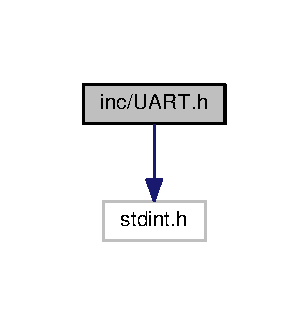
\includegraphics[width=148pt]{UART_8h__incl}
\end{center}
\end{figure}
\subsection*{Macros}
\begin{DoxyCompactItemize}
\item 
\#define {\bfseries CR}~0x0D\hypertarget{UART_8h_a876ce77f3c672c7162658151e648389e}{}\label{UART_8h_a876ce77f3c672c7162658151e648389e}

\item 
\#define {\bfseries LF}~0x0A\hypertarget{UART_8h_a350c9d6cb81908d59427ee96844d1a9c}{}\label{UART_8h_a350c9d6cb81908d59427ee96844d1a9c}

\item 
\#define {\bfseries BS}~0x08\hypertarget{UART_8h_a580a88f98668df1ac5e1683cae31c0b3}{}\label{UART_8h_a580a88f98668df1ac5e1683cae31c0b3}

\item 
\#define {\bfseries E\+SC}~0x1B\hypertarget{UART_8h_a4af1b6159e447ba72652bb7fcdfa726e}{}\label{UART_8h_a4af1b6159e447ba72652bb7fcdfa726e}

\item 
\#define {\bfseries SP}~0x20\hypertarget{UART_8h_aecd69d9a67487cc45c38eb184c50538a}{}\label{UART_8h_aecd69d9a67487cc45c38eb184c50538a}

\item 
\#define {\bfseries D\+EL}~0x7F\hypertarget{UART_8h_ad1e508e805e4ddbc05119be4bb260985}{}\label{UART_8h_ad1e508e805e4ddbc05119be4bb260985}

\end{DoxyCompactItemize}
\subsection*{Functions}
\begin{DoxyCompactItemize}
\item 
void \hyperlink{UART_8h_ad5cbed2a2222bb84e8b5c1caaa50634e}{U\+A\+R\+T\+\_\+\+Init} (void)\hypertarget{UART_8h_ad5cbed2a2222bb84e8b5c1caaa50634e}{}\label{UART_8h_ad5cbed2a2222bb84e8b5c1caaa50634e}

\begin{DoxyCompactList}\small\item\em Initialize the U\+A\+RT for 115,200 baud rate (assuming 50 M\+Hz clock), 8 bit word length, no parity bits, one stop bit, F\+I\+F\+Os enabled. \end{DoxyCompactList}\item 
char \hyperlink{UART_8h_a00e894bb188320a2f4dcd5a78b80da52}{U\+A\+R\+T\+\_\+\+In\+Char} (void)
\begin{DoxyCompactList}\small\item\em Wait for new serial port input. \end{DoxyCompactList}\item 
void \hyperlink{UART_8h_a4ef2f92682b12a347cf1f81cccda4da7}{U\+A\+R\+T\+\_\+\+Out\+Char} (char data)
\begin{DoxyCompactList}\small\item\em 8-\/bit to serial port \end{DoxyCompactList}\item 
void \hyperlink{UART_8h_a2cbbed822dc8e6d801e6c9f21a2cd418}{U\+A\+R\+T\+\_\+\+Out\+String} (char $\ast$pt)
\begin{DoxyCompactList}\small\item\em Output String (N\+U\+LL termination) \end{DoxyCompactList}\item 
uint32\+\_\+t \hyperlink{UART_8h_a0a28a219c31df1bd2182e4b3afbcc5cd}{U\+A\+R\+T\+\_\+\+In\+U\+Dec} (void)
\begin{DoxyCompactList}\small\item\em In\+U\+Dec accepts A\+S\+C\+II input in unsigned decimal format and converts to a 32-\/bit unsigned number valid range is 0 to 4294967295 (2$^\wedge$32-\/1) If you enter a number above 4294967295, it will return an incorrect value Backspace will remove last digit typed. \end{DoxyCompactList}\item 
void \hyperlink{UART_8h_a9a53c5fe8486e0282990b11a218c2625}{U\+A\+R\+T\+\_\+\+Out\+U\+Dec} (uint32\+\_\+t n)
\begin{DoxyCompactList}\small\item\em Output a 32-\/bit number in unsigned decimal format. \end{DoxyCompactList}\item 
uint32\+\_\+t \hyperlink{UART_8h_a5a7efc717f2c844f08689418dd50ee43}{U\+A\+R\+T\+\_\+\+In\+U\+Hex} (void)
\begin{DoxyCompactList}\small\item\em Accepts A\+S\+C\+II input in unsigned hexadecimal (base 16) format No \textquotesingle{}\$\textquotesingle{} or \textquotesingle{}0x\textquotesingle{} need be entered, just the 1 to 8 hex digits It will convert lower case a-\/f to uppercase A-\/F and converts to a 16 bit unsigned number value range is 0 to F\+F\+F\+F\+F\+F\+FF If you enter a number above F\+F\+F\+F\+F\+F\+FF, it will return an incorrect value Backspace will remove last digit typed. \end{DoxyCompactList}\item 
void \hyperlink{UART_8h_a21661aabfda94ec88e9514856f062a41}{U\+A\+R\+T\+\_\+\+Out\+U\+Hex} (uint32\+\_\+t number)
\begin{DoxyCompactList}\small\item\em Output a 32-\/bit number in unsigned hexadecimal format Variable format 1 to 8 digits with no space before or after. \end{DoxyCompactList}\item 
void \hyperlink{UART_8h_a4278ab3463fadff60a5a84792707c3a3}{U\+A\+R\+T\+\_\+\+In\+String} (char $\ast$buf\+Pt, uint16\+\_\+t max)
\begin{DoxyCompactList}\small\item\em Accepts A\+S\+C\+II characters from the serial port and adds them to a string until $<$enter$>$ is typed or until max length of the string is reached. It echoes each character as it is inputted. If a backspace is inputted, the string is modified and the backspace is echoed terminates the string with a null character uses busy-\/waiting synchronization on R\+D\+RF Modified by Agustinus Darmawan + Mingjie Qiu. \end{DoxyCompactList}\item 
void \hyperlink{UART_8h_a7951d2bd4596b8398c204cc7292cf668}{U\+A\+R\+T\+\_\+set\+Redirect} (char $\ast$F)
\begin{DoxyCompactList}\small\item\em Accept Filename and make it as redirect file. \end{DoxyCompactList}\item 
void \hyperlink{UART_8h_ae3522f1847db40b20a24172b5c6f224b}{U\+A\+R\+T\+\_\+end\+Redirect} ()\hypertarget{UART_8h_ae3522f1847db40b20a24172b5c6f224b}{}\label{UART_8h_ae3522f1847db40b20a24172b5c6f224b}

\begin{DoxyCompactList}\small\item\em End redirection. \end{DoxyCompactList}\end{DoxyCompactItemize}


\subsection{Detailed Description}
Runs on L\+M4\+F120/\+T\+M4\+C123 Use U\+A\+R\+T0 to implement bidirectional data transfer to and from a computer running Hyper\+Terminal. This time, interrupts and F\+I\+F\+Os are used. 

\begin{DoxyAuthor}{Author}
Daniel Valvano 
\end{DoxyAuthor}


\subsection{Function Documentation}
\index{U\+A\+R\+T.\+h@{U\+A\+R\+T.\+h}!U\+A\+R\+T\+\_\+\+In\+Char@{U\+A\+R\+T\+\_\+\+In\+Char}}
\index{U\+A\+R\+T\+\_\+\+In\+Char@{U\+A\+R\+T\+\_\+\+In\+Char}!U\+A\+R\+T.\+h@{U\+A\+R\+T.\+h}}
\subsubsection[{\texorpdfstring{U\+A\+R\+T\+\_\+\+In\+Char(void)}{UART_InChar(void)}}]{\setlength{\rightskip}{0pt plus 5cm}char U\+A\+R\+T\+\_\+\+In\+Char (
\begin{DoxyParamCaption}
\item[{void}]{}
\end{DoxyParamCaption}
)}\hypertarget{UART_8h_a00e894bb188320a2f4dcd5a78b80da52}{}\label{UART_8h_a00e894bb188320a2f4dcd5a78b80da52}


Wait for new serial port input. 

\begin{DoxyReturn}{Returns}
char A\+S\+C\+II code for key typed 
\end{DoxyReturn}
\index{U\+A\+R\+T.\+h@{U\+A\+R\+T.\+h}!U\+A\+R\+T\+\_\+\+In\+String@{U\+A\+R\+T\+\_\+\+In\+String}}
\index{U\+A\+R\+T\+\_\+\+In\+String@{U\+A\+R\+T\+\_\+\+In\+String}!U\+A\+R\+T.\+h@{U\+A\+R\+T.\+h}}
\subsubsection[{\texorpdfstring{U\+A\+R\+T\+\_\+\+In\+String(char $\ast$buf\+Pt, uint16\+\_\+t max)}{UART_InString(char *bufPt, uint16_t max)}}]{\setlength{\rightskip}{0pt plus 5cm}void U\+A\+R\+T\+\_\+\+In\+String (
\begin{DoxyParamCaption}
\item[{char $\ast$}]{buf\+Pt, }
\item[{uint16\+\_\+t}]{max}
\end{DoxyParamCaption}
)}\hypertarget{UART_8h_a4278ab3463fadff60a5a84792707c3a3}{}\label{UART_8h_a4278ab3463fadff60a5a84792707c3a3}


Accepts A\+S\+C\+II characters from the serial port and adds them to a string until $<$enter$>$ is typed or until max length of the string is reached. It echoes each character as it is inputted. If a backspace is inputted, the string is modified and the backspace is echoed terminates the string with a null character uses busy-\/waiting synchronization on R\+D\+RF Modified by Agustinus Darmawan + Mingjie Qiu. 


\begin{DoxyParams}{Parameters}
{\em buf\+Pt} & pointer to empty buffer \\
\hline
{\em max} & size of buffer \\
\hline
\end{DoxyParams}
\index{U\+A\+R\+T.\+h@{U\+A\+R\+T.\+h}!U\+A\+R\+T\+\_\+\+In\+U\+Dec@{U\+A\+R\+T\+\_\+\+In\+U\+Dec}}
\index{U\+A\+R\+T\+\_\+\+In\+U\+Dec@{U\+A\+R\+T\+\_\+\+In\+U\+Dec}!U\+A\+R\+T.\+h@{U\+A\+R\+T.\+h}}
\subsubsection[{\texorpdfstring{U\+A\+R\+T\+\_\+\+In\+U\+Dec(void)}{UART_InUDec(void)}}]{\setlength{\rightskip}{0pt plus 5cm}uint32\+\_\+t U\+A\+R\+T\+\_\+\+In\+U\+Dec (
\begin{DoxyParamCaption}
\item[{void}]{}
\end{DoxyParamCaption}
)}\hypertarget{UART_8h_a0a28a219c31df1bd2182e4b3afbcc5cd}{}\label{UART_8h_a0a28a219c31df1bd2182e4b3afbcc5cd}


In\+U\+Dec accepts A\+S\+C\+II input in unsigned decimal format and converts to a 32-\/bit unsigned number valid range is 0 to 4294967295 (2$^\wedge$32-\/1) If you enter a number above 4294967295, it will return an incorrect value Backspace will remove last digit typed. 

\begin{DoxyReturn}{Returns}
uint32\+\_\+t 32-\/bit unsigned number 
\end{DoxyReturn}
\index{U\+A\+R\+T.\+h@{U\+A\+R\+T.\+h}!U\+A\+R\+T\+\_\+\+In\+U\+Hex@{U\+A\+R\+T\+\_\+\+In\+U\+Hex}}
\index{U\+A\+R\+T\+\_\+\+In\+U\+Hex@{U\+A\+R\+T\+\_\+\+In\+U\+Hex}!U\+A\+R\+T.\+h@{U\+A\+R\+T.\+h}}
\subsubsection[{\texorpdfstring{U\+A\+R\+T\+\_\+\+In\+U\+Hex(void)}{UART_InUHex(void)}}]{\setlength{\rightskip}{0pt plus 5cm}uint32\+\_\+t U\+A\+R\+T\+\_\+\+In\+U\+Hex (
\begin{DoxyParamCaption}
\item[{void}]{}
\end{DoxyParamCaption}
)}\hypertarget{UART_8h_a5a7efc717f2c844f08689418dd50ee43}{}\label{UART_8h_a5a7efc717f2c844f08689418dd50ee43}


Accepts A\+S\+C\+II input in unsigned hexadecimal (base 16) format No \textquotesingle{}\$\textquotesingle{} or \textquotesingle{}0x\textquotesingle{} need be entered, just the 1 to 8 hex digits It will convert lower case a-\/f to uppercase A-\/F and converts to a 16 bit unsigned number value range is 0 to F\+F\+F\+F\+F\+F\+FF If you enter a number above F\+F\+F\+F\+F\+F\+FF, it will return an incorrect value Backspace will remove last digit typed. 

\begin{DoxyReturn}{Returns}
uint32\+\_\+t 32-\/bit unsigned number 
\end{DoxyReturn}
\index{U\+A\+R\+T.\+h@{U\+A\+R\+T.\+h}!U\+A\+R\+T\+\_\+\+Out\+Char@{U\+A\+R\+T\+\_\+\+Out\+Char}}
\index{U\+A\+R\+T\+\_\+\+Out\+Char@{U\+A\+R\+T\+\_\+\+Out\+Char}!U\+A\+R\+T.\+h@{U\+A\+R\+T.\+h}}
\subsubsection[{\texorpdfstring{U\+A\+R\+T\+\_\+\+Out\+Char(char data)}{UART_OutChar(char data)}}]{\setlength{\rightskip}{0pt plus 5cm}void U\+A\+R\+T\+\_\+\+Out\+Char (
\begin{DoxyParamCaption}
\item[{char}]{data}
\end{DoxyParamCaption}
)}\hypertarget{UART_8h_a4ef2f92682b12a347cf1f81cccda4da7}{}\label{UART_8h_a4ef2f92682b12a347cf1f81cccda4da7}


8-\/bit to serial port 


\begin{DoxyParams}{Parameters}
{\em data} & letter is an 8-\/bit A\+S\+C\+II character to be transferred \\
\hline
\end{DoxyParams}
\index{U\+A\+R\+T.\+h@{U\+A\+R\+T.\+h}!U\+A\+R\+T\+\_\+\+Out\+String@{U\+A\+R\+T\+\_\+\+Out\+String}}
\index{U\+A\+R\+T\+\_\+\+Out\+String@{U\+A\+R\+T\+\_\+\+Out\+String}!U\+A\+R\+T.\+h@{U\+A\+R\+T.\+h}}
\subsubsection[{\texorpdfstring{U\+A\+R\+T\+\_\+\+Out\+String(char $\ast$pt)}{UART_OutString(char *pt)}}]{\setlength{\rightskip}{0pt plus 5cm}void U\+A\+R\+T\+\_\+\+Out\+String (
\begin{DoxyParamCaption}
\item[{char $\ast$}]{pt}
\end{DoxyParamCaption}
)}\hypertarget{UART_8h_a2cbbed822dc8e6d801e6c9f21a2cd418}{}\label{UART_8h_a2cbbed822dc8e6d801e6c9f21a2cd418}


Output String (N\+U\+LL termination) 


\begin{DoxyParams}{Parameters}
{\em pt} & pointer to a N\+U\+L\+L-\/terminated string to be transferred \\
\hline
\end{DoxyParams}
\index{U\+A\+R\+T.\+h@{U\+A\+R\+T.\+h}!U\+A\+R\+T\+\_\+\+Out\+U\+Dec@{U\+A\+R\+T\+\_\+\+Out\+U\+Dec}}
\index{U\+A\+R\+T\+\_\+\+Out\+U\+Dec@{U\+A\+R\+T\+\_\+\+Out\+U\+Dec}!U\+A\+R\+T.\+h@{U\+A\+R\+T.\+h}}
\subsubsection[{\texorpdfstring{U\+A\+R\+T\+\_\+\+Out\+U\+Dec(uint32\+\_\+t n)}{UART_OutUDec(uint32_t n)}}]{\setlength{\rightskip}{0pt plus 5cm}void U\+A\+R\+T\+\_\+\+Out\+U\+Dec (
\begin{DoxyParamCaption}
\item[{uint32\+\_\+t}]{n}
\end{DoxyParamCaption}
)}\hypertarget{UART_8h_a9a53c5fe8486e0282990b11a218c2625}{}\label{UART_8h_a9a53c5fe8486e0282990b11a218c2625}


Output a 32-\/bit number in unsigned decimal format. 


\begin{DoxyParams}{Parameters}
{\em n} & 32-\/bit number to be transferred \\
\hline
\end{DoxyParams}
\index{U\+A\+R\+T.\+h@{U\+A\+R\+T.\+h}!U\+A\+R\+T\+\_\+\+Out\+U\+Hex@{U\+A\+R\+T\+\_\+\+Out\+U\+Hex}}
\index{U\+A\+R\+T\+\_\+\+Out\+U\+Hex@{U\+A\+R\+T\+\_\+\+Out\+U\+Hex}!U\+A\+R\+T.\+h@{U\+A\+R\+T.\+h}}
\subsubsection[{\texorpdfstring{U\+A\+R\+T\+\_\+\+Out\+U\+Hex(uint32\+\_\+t number)}{UART_OutUHex(uint32_t number)}}]{\setlength{\rightskip}{0pt plus 5cm}void U\+A\+R\+T\+\_\+\+Out\+U\+Hex (
\begin{DoxyParamCaption}
\item[{uint32\+\_\+t}]{number}
\end{DoxyParamCaption}
)}\hypertarget{UART_8h_a21661aabfda94ec88e9514856f062a41}{}\label{UART_8h_a21661aabfda94ec88e9514856f062a41}


Output a 32-\/bit number in unsigned hexadecimal format Variable format 1 to 8 digits with no space before or after. 


\begin{DoxyParams}{Parameters}
{\em number} & 32-\/bit number to be transferred \\
\hline
\end{DoxyParams}
\index{U\+A\+R\+T.\+h@{U\+A\+R\+T.\+h}!U\+A\+R\+T\+\_\+set\+Redirect@{U\+A\+R\+T\+\_\+set\+Redirect}}
\index{U\+A\+R\+T\+\_\+set\+Redirect@{U\+A\+R\+T\+\_\+set\+Redirect}!U\+A\+R\+T.\+h@{U\+A\+R\+T.\+h}}
\subsubsection[{\texorpdfstring{U\+A\+R\+T\+\_\+set\+Redirect(char $\ast$\+F)}{UART_setRedirect(char *F)}}]{\setlength{\rightskip}{0pt plus 5cm}void U\+A\+R\+T\+\_\+set\+Redirect (
\begin{DoxyParamCaption}
\item[{char $\ast$}]{F}
\end{DoxyParamCaption}
)}\hypertarget{UART_8h_a7951d2bd4596b8398c204cc7292cf668}{}\label{UART_8h_a7951d2bd4596b8398c204cc7292cf668}


Accept Filename and make it as redirect file. 


\begin{DoxyParams}{Parameters}
{\em string} & of filename \\
\hline
\end{DoxyParams}

%--- End generated contents ---

% Index
\backmatter
\newpage
\phantomsection
\clearemptydoublepage
\addcontentsline{toc}{chapter}{Index}
\printindex

\end{document}
